\minitoc

\vspace{0.5cm}
The second chapter focuses on the most fundamental decision unit of microeconomic theory: \textit{consumer}. The main reference is Chapter 2 and 3 of \citet{mas1995microeconomic}.

The basic setting of consumer demand study is \textit{market economy}, where the goods and services that the consumer may acquire and consume are available for purchase at known prices (or trade for other goods at know exchange rates).

In this chapter, we will focus on 2 major aspects of the consumer theory: choice and demand.
\begin{center}
    \begin{tabular}{rl}
    \hline
    \textbf{choice} & individual decision making analysis based on choice\\ 
    \textbf{demand} & individual decision making analysis based on preference \\ 
    \hline
    \end{tabular}
\end{center}

The starting point of individual decision problem is a \textit{set of possible (mutually exclusive) alternatives} from which the individual must choose. To model decision making process
on this set of alternatives, one can:
\begin{enumerate}
    \item[-] either start from the tastes, i.e., \textit{preference relations} of individuals, and set up the patterns of decision making with preferences
    \item[-] or, start from the actual actions of individuals, i.e. \textit{choices}, to deduct a pattern of decision making
\end{enumerate}

The two aspects of consumer theory are actually closely related to each other. Just like choices and preferences in Chapter 1, they are two sides of the same coin. However, they are NOT equivalent.
The major conclusion of choice-based consumer theory is WARP is essentially equivalent to the \textit{compensated law of demand}, but WARP imposes fewer restrictions on demand than preference-based theory,
hence, does NOT necessarily guarantee the existence of a rationalizing preference relation for consumer demand, therefore, \textit{strong axiom of revealed preference} is introduced.

\section{Basic Setting}\label{chap2:sec1}
First, we introduce the basic settings of a consumer's problem in a market economy. These concepts will keep reoccuring in the following sections.

\subsection{Commodities}\label{chap2:sec1:ssec1}
First, we need to define the goods and services the consumers consume. We do not actually care about what they specifically are, instead, we use a very abstract concept \textit{commodities}
to summarize and analyze them.
\begin{definition}{commodity bundle}{}
    Assume there are $L<\infty$ different commodities, a \textit{commodity vector} or \textit{commodity bundle} is a list of amounts of the different commodities:$$x=\left[x_1,\cdots,x_L\right]^T$$
\end{definition}
$x$ can be view as a point in an $\mathbb{R}^L$ space, i.e., the commodity space. Each entry $x_l$ of $x$ ($l=1,\cdots,L$) represents the amount of commodity $l$ consumed, hence, the vector is referred to
as \textit{consumption vector} or \textit{consumption bundle}.

Three things to keep in mind:
\begin{enumerate}
    \item[-] Time can be incorporated into this setting, namely, today's commodity is distinct from tomorrow's commodity, even if they are otherwise the same. The value of time will come back in later chapters and is crucial in a large strand of behavioral economic literature. Same logic applies to other limitations that are easily neglected, like geographic ones.
    \item[-] Negative entries can exists in a commodity vector, indicating debits or net outflows of goods. In a producing problem or exchange problem, negative entries of commodity vectors are not rare.
    \item[-] Consumption is quite flexible and comes in many format empirically, for the sake of data collection conveniency, consumption data are often aggregated monthly, quarterly for even annually. Meanwhle, some consumptions in the commodity vectors may not actually occur in the market.
\end{enumerate}

\subsection{The Consumption Set}\label{chap2:sec1:ssec2}
Consumptions are limited by a number of constraints, which will form a subset of commodity space $X\subset \mathcal{R}^L$. With in this subset, all possible commodity bundles can be 
consumed, this is exactly the definition of consumption sets (see \citet[Page 19-20]{mas1995microeconomic} for some simple examples of consumption sets).

For now, we will focus on the simplest consumption set: all possible non-negative commodity bundles:
$$X=\mathbb{R}^L_+=\{x\in \mathbb{R}^L: x_l\geq 0,\forall l=1,\cdots, L\}$$

It is easy to show that
$$\mathbb{R}^L_+ \text{ is a }\textbf{convex} \text{ set}$$

A brief proof: $\forall \vec{x},\vec{y}\in \mathbb{R}^L_+$ and $\forall\alpha \in [0,1]$, $\alpha\vec{x}+(1-\alpha)\vec{y}=[\alpha x_1+(1-\alpha)y_1,\cdots,$ $\alpha x_L+(1-\alpha)y_L]^T$. Since $x_i\geq 0,y_i\geq 0$, $\alpha x_i+(1-\alpha)y_i\geq 0 \Rightarrow\alpha\vec{x}+(1-\alpha)\vec{y}\in \mathbb{R}^L_+$.

Convexity of consumption sets is an essential assumption here, but some of the results do survive without the assumption fo convexity.

Although consuption sets are formed due to some constraints, but these constraints have nothing to do with consumers' budget (exogenous constraints). It is intuitive that with a large enough budget (infinitely large if you may), you can always afford any consumption bundle in a give consumption set. But what if consumers, as in reality, do have a budget constraint and cannot afford every bundle in the consumption set?

\subsection{Prices and Consumption Cost}\label{chap2:sec1:ssec3}
Budget constraints are an important economic constraint faced by consumers: one can only consume the commodity bundles that she can afford.

To formalize this constraint, we need to introduce the \textit{price vector}: 
$$\vec{p}=\left[p_1,\cdots,p_L\right]\in \mathbb{R}^L$$
This price vector contains unit price information for each of the $L$ commodities. They are all traded in the market and the price information of them is publicly quoted (the \textit{principle of completeness of markets}).
For simplicity, we assume $\vec{p}\gg 0$ i.e. $\forall l,p_l>0$\footnote{Of course, price can be negative, meaning that consumers are actually paid to consume the "bad "commodity, such as polution.}.

Another important assumption is the \textit{price-taking assumption}: consumers do NOT have the power to influence the prices. Here, each consumer only buys a small (neglectable) fraction of the total demand for commodities.

With prices defined, we can finally define the \textbf{economic-affordability constraint} of consumers: For a consumer with wealth $w$, a consumption bundle $\vec{x}\in \mathbb{R}^L_+$ is affordable if its total cost does NOT exceed the consumer's wealth level $w$, formally, $$\vec{p}\cdot \vec{x}=p_1x_1+p_2x_2+\cdots+p_Lx_L\leq w$$
With the two core assumptions stated above, consumers face a \textit{linear price schedule}.

\section{Choice Based Consumer Theory}\label{chap2:sec2}
\subsection{Walrasian Budgets}
We have already defined the economic-affordability constraint of consumers, if we also limit consumption bundle $x$ to be non-negative, we would have the Walrasian, or competitive budget:

\begin{definition}
    The Walrasian, or competitive budget set $$B_{\mathbf{p},w}=\{x\in\mathbb{R}^L_+:\mathbf{p}\cdot\mathbf{x}\leq w\}$$ is the set of all feasible consumption bundles give market prices $\mathbf{p}$ and wealth $w$.
\end{definition}

From a Walrasian budget's point of view, a consumer can only choose a consumption bundle $x$ from $B_{\mathbf{p},w}$. An underlining assumption here is $w>0$, otherwise consumers cannot afford anything. We can also
separately define the "edge" of a Walrasian budget set as:
\begin{definition}
    The \textit{budget hyperplane} is the set $\{x\in\mathbb{R}^L_+:\mathbf{p}\cdot\mathbf{x}=w\}$
\end{definition}
It determines the upper bound of the budget set: with prices of other commodities ($\mathbf{p}_{-i}$) and wealth level $w$ fixed, the change of commodity $i$'s price $p_i$ will enlarge/shrink the budget set by moving the budget hyperplane.
Geometrically, the price vector $\mathbf{p}$ must be orthogonal to the budget hyperplane, we can think it this way: for any two bundles $\mathbf{x}$ and $\mathbf{x}'$ one the budget hyperplane, we must have $\mathbf{p}\cdot\mathbf{x}=\mathbf{p}\cdot\mathbf{x}'=w$, hence
$\mathbf{p}\cdot\Delta\mathbf{x}=\mathbf{p}\cdot(\mathbf{x}'-\mathbf{x})=0$ is always true.

A core feature of the Walrasian budget set is that it is \textbf{convex}: $\forall \mathbf{x},\mathbf{y}\in B_{\mathbf{p},w}, \alpha\in[0,1], \alpha\mathbf{x}+(1-\alpha)\mathbf{y}\in B_{\mathbf{p},w}$. This is very easy to prove: $\mathbf{x}\in\mathbb{R}^L_+\land\mathbf{y}\in\mathbb{R}^L_+\Rightarrow \alpha\mathbf{x}+(1-\alpha)\mathbf{y}\in \mathbb{R}^L_+$, $\mathbf{p}\cdot\mathbf{x}\leq w\land\mathbf{p}\cdot \mathbf{y}\leq w\Rightarrow \alpha(\mathbf{p}\cdot\mathbf{x})+(1-\alpha)(\mathbf{p}\cdot\mathbf{y})\leq w$.
Notice that the Walrasian budget set is not automatically convex. Its convexity is induced from the convexity of its superset (the consumption set), in this case $\mathbb{R}^L_+$. In general, it is easy to show that the Walrasian budget set will convex as long as its corresponding consumption set is convex.

Of course, it is perfectly possible that a consumer's budget is NOT convex (and not Walrasian, in that sense), the brilliant work of \citet{deaton1980economics} has documented and discussed many complicated consumption sets that are not convex.

\subsection{Walrasian Demand Function}
With Walrasian budgets defined, we can define \textit{Walrasian demand correspondence} and \textit{Walrasian demand function} as:
\begin{definition}
    For each \textit{price-wealth} pair $(\mathbf{p},w)$, Walrasian demand correspondence is the set of chosen consumption bundles, written as $\mathbf{x}(\mathbf{p},w)$. When $\mathbf{x}(\mathbf{p},w)$ is single-valued, it will be referred to as a \textbf{Walrasian demand function}.
\end{definition}

The two main assumptions of $\mathbf{x}(\mathbf{p},w)$ are:
\begin{definition}
    For a Walrasian demand correspondence $\mathbf{x}(\mathbf{p},w)$, we assume it is:
    \begin{enumerate}
        \item[1.] \textbf{Homogeneous of degree zero}: $\forall \mathbf{p},w$ and $\alpha >0$, $\mathbf{x}(\alpha \mathbf{p},\alpha w)=\mathbf{x}(\mathbf{p},w)$. This means that if wealth and prices change in the same proportion at the same time, consumer would not change her choice. 
        
        There are two implications of homogeneous of degree zero assumption:
        \begin{enumerate}
            \item[-] \textbf{Dimension reduction}: With this assumption, we can reduce $\mathbf{x}(\mathbf{p},w)$ to $\mathbf{x}(\tilde{\mathbf{p}},1)$ where $\tilde{\mathbf{p}}=\frac{1}{w}\mathbf{p}$, hence to a $L$-argument problem.
            \item[-] \textbf{Choice structure}: By homogeneity of degree zero, $\mathbf{x}(\mathbf{p},w)$ depends only on $\mathbf{p}$ and $w$, i.e. the budget set, then for the family of Walrasian budget sets $\mathcal{B}^*=\{B_{\mathbf{p},w}:\mathbf{p}\gg 0,w>0\}$, $(\mathcal{B}^*,\mathbf{x}(\cdot))$ is a choice structure. This choice structure does NOT include all possible subsets of $X$\sidenotes{$\leftarrow X$ is the set of all possible bundles}, in particular, not all two- and three-element subsets of $X$\footnote{This relates to the argument that when one consumption bundle $\mathbf{x^*}$ is infeasible, it not being chosen does NOT mean it is less preferred. This will be dealt with more carefully with more assumptions of preference-based demand.}, therefore, requires more assumptions to have a rationalizing preference.
        \end{enumerate}
             
        \item[2.] \textbf{Walras' law}: $\forall \gg 0,w>0$, $\mathbf{p}\cdot\mathbf{x}=w$ for every $\mathbf{x}\in \mathbf{x}(\mathbf{p},w)$. Walras' law means that a consumer want to spend all her wealth for consumption, every consumption bundle hence will exhaust $w$. Walras' law implies that goods are continuous.
        
        Notice that this is implicitly intertemporal, meaning that Walras' law consider lifetime resource allocation.
    \end{enumerate}
\end{definition}

Next, we disucess several basic definitions induced from the Walrasian demand function. For a demand function 
$$\mathbf{x}(\mathbf{p},w)=\left[x_1 (\mathbf{p},w),x_2 (\mathbf{p},w),\cdots, x_L(\mathbf{p},w) \right]^T$$ we have the following two effects:

\begin{description}
    \item[Wealth effects] \underline{Fix $\mathbf{p}$, get a function of $x(w)$}.
    
    Take the partial derivative of demand function on wealth: $$D_w x(\mathbf{x},w)=\left[\frac{\partial x_1(\mathbf{p},w)}{\partial w}, \frac{\partial x_2(\mathbf{p},w)}{\partial w},\cdots, \frac{\partial x_L(\mathbf{p},w)}{\partial w} \right]^T$$, then $\frac{\partial x_l(\mathbf{p},w)}{\partial w}$ is the \textit{wealth effect} for the $l$th commodity.
    Wealth effects can classify commodities into two types:
    \begin{enumerate}
        \item[-] \textbf{normal}: $\partial x_l(\mathbf{p},w)/\partial w\geq 0$
        \item[-] \textbf{inferior}: $\partial x_l(\mathbf{p},w)/\partial w <0$
    \end{enumerate} 
    \item[Price effects] \underline{For commodity $l$, fix $\mathbf{p}_{-l}$ and $w$, get a function of $x(p_l)$}.
    
    Take the partial derivative of demand function on price vector:
    $$D_{\mathbf{p}}x(\mathbf{p},w)= \begin{bmatrix}
        \nabla_{\mathbf{p}}x_1(\mathbf{p},w)\\
        \vdots\\
        \nabla_{\mathbf{p}}x_L(\mathbf{p},w) \end{bmatrix} 
    =
    \begin{bmatrix}
        \frac{\partial x_1(\mathbf{p},w)}{\partial p_1} & \cdots & \frac{\partial x_1(\mathbf{p},w)}{\partial p_L}\\
        \vdots & \ddots & \vdots\\
        \frac{\partial x_L(\mathbf{p},w)}{\partial p_1} & \cdots &\frac{\partial x_L(\mathbf{p},w)}{\partial p_L}
        \end{bmatrix}$$
\end{description}

For most goods, the price effects would be negative: you would buy more if the price is lower. However, there \textit{Giffen} goods (often low quality) and \textit{Veblen} goods (often luxurious) that have positive price effects.

Regarding wealth effects $\partial x_l(\mathbf{p},w)/partial w$ and price effects $\partial x_l(\mathbf{p},w)/\partial p_k$, we have the following two theorems:

\begin{theorem}\label{thm_homo_waldemand_thm1}
    If the Walrasian demand function $\mathbf{x}(\mathbf{p},w)$ is \textbf{homogeneous of degree zero}, the $\forall \mathbf{p},w$:
    $$\sum^L_{k=1}\frac{\partial x_l(\mathbf{p},w)}{\partial p_k}p_k +\frac{\partial x_l(\mathbf{p},w)}{\partial w}w=0,\forall l=1,\cdots,L$$
\end{theorem}

This is easy to proof: homogeneity of degree zero gives $\mathbf{x}(\alpha \mathbf{p},\alpha w)-\mathbf{x}(\mathbf{p},w)=0$, differentiating with respect to $\alpha$, get:
$$D_{\alpha \mathbf{p}}\mathbf{x}(\alpha \mathbf{p},\alpha w)\cdot \mathbf{p} + D_{\alpha w} \mathbf{x}(\alpha \mathbf{p},\alpha w)w=0$$
this is true for any $\alpha$, if we take $\alpha=1$, we get $D_{\mathbf{p}}\mathbf{x}(\mathbf{p}, w)\cdot \mathbf{p} + D_{ w} \mathbf{x}( \mathbf{p}, w)w=\mathbf{0}$, which is just the matrix notation of Thm.\ref{thm_homo_waldemand_thm1}.

Intuitively, this implies the price (substitution) effects and wealth (income) effects induced by the price change of one commodity, when weighted by the prices of other commodities and wealth, will cancel out.

Another theorem is induced from Walras' law:
\begin{theorem}\label{thm_walraslaw_waldemand_thm2}
    If the Walrasian emand function $\mathbf{x}(\mathbf{p},w)$ satisfies \textbf{Walras' law}, then for all $\mathbf{p},w$:
    $$\sum^L_{l=1}p_l\frac{\partial x_l(\mathbf{p},w)}{\partial p_k}+x_k(\mathbf{p},w)=0,\forall k=1,\cdots,L$$
    and
    $$\sum^L_{l=1}p_l\frac{\partial x_l(\mathbf{p},w)}{\partial w}=1$$
\end{theorem}

The proof is also easy: Walras' law gives $\mathbf{p}\cdot \mathbf{x}(\mathbf{p},w)=w$, take derivatives with respect to $\mathbf{p}$, get $\mathbf{p}\cdot D_{\mathbf{p}}\mathbf{x}(\mathbf{p},w)+\mathbf{x}(\mathbf{p},w)^T=\mathbf{0}^T$; take derivatives with repsect to $w$, get $\mathbf{p}\cdot D_{w}(\mathbf{p},w)=1$. The intuition is: a change in prices do NOT change the total expenditure, and the total expenditure will change by the same amount with the change in wealth.

If we define elasticities as:
\begin{align*} 
    \epsilon_{lk}=\frac{\partial x_l(\mathbf{p},w)/x_l(\mathbf{p},w)}{\partial p_k /p_k} && \text{ \% change in demand for $l$ per \% change in the price of $k$} \\ 
    \epsilon_{lw}=\frac{\partial x_l(\mathbf{p},w)/x_l(\mathbf{p},w)}{\partial w/w} && \text{ \% change in demand for $l$ per \% change in wealth $w$}
\end{align*}

We can rewrite Thm.\ref{thm_homo_waldemand_thm1} as $\sum^L_{k=1}\epsilon_{lk}(\mathbf{p},w)+\epsilon_{lw}(\mathbf{p},w)=0$ for $l=1,\cdots,L$: this directly expresses that an equal \% change in all prices and wealth leads to no change in demand, i.e., the homogeneity of degree zero.
And we can rewrite the two equations in Thm.\ref{thm_walraslaw_waldemand_thm2} as $\sum^L_{l=1}\frac{p_lx_l(\mathbf{p},w)}{w}\epsilon_{lk}(\mathbf{p},w)+\frac{p_kx_k(\mathbf{p},w)}{w}=0$ for $k=1,\cdots,L$ and $\sum^L_{l=1}\frac{p_lx_l(\mathbf{p},w)}{w}\epsilon_{lw}(\mathbf{p},w)=1$.

\subsection{WARP and Law of Demand}
Since for the family of Walrasian budget sets $\mathcal{B}^*=\{B_{\mathbf{p},w}:\mathbf{p}\gg 0,w>0\}$, $(\mathcal{B}^*,\mathbf{p}(\cdot))$ is a choice structure, naturally, we would like to check when WARP holds for this choice structure.

\begin{definition}\label{def_walrasian_WARP}
    A Walrasian demand function $\mathbf{x}(\mathbf{p},w)$ satisfies WARP if any two price-wealth conditions $(\mathbf{p},w)$ and $(\mathbf{p}',w')$ satisfies:
    $$\mathbf{p}\cdot \mathbf{x}(\mathbf{p}',w')\leq w\text{ and }\mathbf{x}(\mathbf{p}',w')\neq \mathbf{x}(\mathbf{p},w)\Rightarrow \mathbf{p}'\cdot\mathbf{x}(\mathbf{p},w)>w'$$
\end{definition}

The intuition is quite straightforward: If $\mathbf{p}\cdot \mathbf{x}(\mathbf{p}',w')\leq w$ and $\mathbf{x}(\mathbf{p}',w')\neq \mathbf{x}(\mathbf{p},w)$, the consumer chooses $\mathbf{x}(\mathbf{p},w)$ even when $\mathbf{x}(\mathbf{p}',w')$ is affordable. Hence, $\mathbf{x}(\mathbf{p},w)$ is preferred over $\mathbf{x}(\mathbf{p}',w')$, which means that the only reason why she chooses $\mathbf{x}(\mathbf{p},w)$ instead of $\mathbf{x}(\mathbf{p}',w')$ is that she can not afford $\mathbf{x}(\mathbf{p},w)$ at $(\mathbf{p}',w')$, i.e. $\mathbf{p}'\mathbf{x}(\mathbf{p},w)>w'$. An easier way to understand WARP is that we \textbf{CANNOT} have both $\mathbf{p}'\cdot \mathbf{x}(\mathbf{p},w)\leq w'$ and $\mathbf{p}\cdot \mathbf{x}(\mathbf{p}',w')\leq w$, unless $\mathbf{x}(\mathbf{p}',w')=\mathbf{x}(\mathbf{p},w)$.

It is easy to show that this definition is a special case of Def.\ref{def_WARP}: here we consider single-valued $C(\cdot)$ (function), then Def.\ref{def_WARP} gives that $\forall B,B'$ and $x,y\in B\cap B'$, $x=C(B),y=C(B')\Rightarrow x\in C(B')\Rightarrow x=y$. Rewrite this in the context of Walrasian demand functions, we have: for any $(\mathbf{p},w),(\mathbf{p}',w')$, if $\mathbf{p}\cdot\mathbf{x}(\mathbf{p}',w')\leq w$ and $\mathbf{p}'\cdot \mathbf{x}(\mathbf{p},w)\leq w'$, then $\mathbf{x}(\mathbf{p},w)=\mathbf{x}(\mathbf{p'},w')$. This is the contrapositive statement of Def.\ref{def_walrasian_WARP}. Hence the two definitions are equivalent.

\subsubsection*{WARP and compensated price changes}
WARP can also be stated in terms of compensated price changes. At $(\mathbf{p},w)$, the consumer chooses $\mathbf{x}(\mathbf{p},w)$, if she still want to afford $\mathbf{x}(\mathbf{p},w)$ at a new price $\mathbf{p}'$, she would need to adjust her wealth to $w'=\mathbf{p}'\cdot \mathbf{x}(\mathbf{p},w)$, this gives \textit{Slutsky wealth compensation} $\Delta w=w'-w=\Delta \mathbf{p}\cdot\mathbf{x}(\mathbf{p},w)=(\mathbf{p}'-\mathbf{p})\mathbf{x}(\mathbf{p},w)$, $\Delta \mathbf{p}$ is referred to as \textit{compensated price changes}. With these concepts defined, WARP implies:
\begin{theorem}\label{thm_WARP_to_lawofdemand}
    For any $\Delta \mathbf{p}$ from initial situation $(\mathbf{p},w)$ to $(\mathbf{p}',w')=(\mathbf{p}',\mathbf{p}'\cdot(\mathbf{x},w))$, if WARP holds, we have
    $$(\mathbf{p}'-\mathbf{p})\cdot[\mathbf{x}(\mathbf{p}',w')-\mathbf{x}(\mathbf{p},w)]\leq 0$$
    with strict inequality unless $\mathbf{x}(\mathbf{p},w)=\mathbf{x}(\mathbf{p}',w')$.
\end{theorem}

Here is a proof: rewrite the left-side, get
$$(\mathbf{p}'-\mathbf{p})\cdot[\mathbf{x}(\mathbf{p}',w')-\mathbf{x}(\mathbf{p},w)]=\mathbf{p}'\cdot[\mathbf{x}(\mathbf{p}',w')-\mathbf{x}(\mathbf{p},w)]-\mathbf{p}\cdot[\mathbf{x}(\mathbf{p}',w')-\mathbf{x}(\mathbf{p},w)]$$
By Walras' law, $\mathbf{p}'\cdot\mathbf{x}(\mathbf{p}',w')=w'$, $\mathbf{p}\cdot \mathbf{x}(\mathbf{p},w)=w$, also by assumption of compensated price changes, $\mathbf{p}'\cdot\mathbf{x}(\mathbf{p},w)=w'$, if if WARP holds, since $\mathbf{x}(\mathbf{p},w)$ is affordable at $(\mathbf{p}',w')$, $\mathbf{x}(\mathbf{p}',w')$ must NOT be affordable at $(\mathbf{p},w)$, i.e., $\mathbf{p}\cdot \mathbf{x}(\mathbf{p}',w')>w$, therefore, we have:
$$(\mathbf{p}'-\mathbf{p})\cdot[\mathbf{x}(\mathbf{p}',w')-\mathbf{x}(\mathbf{p},w)]= \underbrace{\mathbf{p}'\cdot[\mathbf{x}(\mathbf{p}',w')-\mathbf{x}(\mathbf{p},w)]}_{=0} - \underbrace{\mathbf{p}\cdot[\mathbf{x}(\mathbf{p}',w')-\mathbf{x}(\mathbf{p},w)]}_{>0}<0$$

This Theorem goes both way, that is
\begin{theorem}\label{thm_lawofdemand_to_WARP}
    If for any compensated price changes, $(\mathbf{p}'-\mathbf{p})\cdot[\mathbf{x}(\mathbf{p}',w')-\mathbf{x}(\mathbf{p},w)]\leq 0$ holds, the WARP is satisfied.
\end{theorem}
We proof the contrapositive: if WARP is violated, there exists a compensated price change such that $(\mathbf{p}'-\mathbf{p})\cdot[\mathbf{x}(\mathbf{p}',w')-\mathbf{x}(\mathbf{p},w)]>0$. A violation of WARP gives that for $(\mathbf{p},w)$ and $(\mathbf{\mathbf{p}',w'})$ such that $\mathbf{x}(\mathbf{p},w)\neq \mathbf{x}(\mathbf{p}',w')$, $\mathbf{p}'\cdot \mathbf{x}(\mathbf{p},w)\leq w'$ and $\mathbf{p}\cdot \mathbf{x}(\mathbf{p}',w')\leq w$ can both be satisfied. The proof is done in 2 steps:
\begin{description}
    \item[Step 1] Prove the fact that: 
    
    If any two price-wealth pairs $(\mathbf{p},w),(\mathbf{p}',w')$, $\mathbf{p}\cdot\mathbf{x}(\mathbf{p}',w')=w,\mathbf{x}(\mathbf{p}',w')\neq \mathbf{x}(\mathbf{p},w)\Rightarrow \mathbf{p}'\cdot \mathbf{x}(\mathbf{p},w)>w'$, then WARP holds. 
    
    Again, we prove the contrapositive of this proposition. Let $(\mathbf{p}',w')$ and $(\mathbf{p}'',w'')$ violates WARP such that $\mathbf{x}(\mathbf{p}',w')\neq \mathbf{x}(\mathbf{p}'',w''),\mathbf{p}'\cdot\mathbf{x}(\mathbf{p}'',w'')\leq w'$ and $\mathbf{p}''\cdot\mathbf{x}(\mathbf{p}',w')\leq w''$. We have two scenarios:
    \begin{enumerate}
        \item[-] $\mathbf{p}'\cdot\mathbf{x}(\mathbf{p}'',w'')= w'$ or $\mathbf{p}''\cdot\mathbf{x}(\mathbf{p}',w')= w''$ or both: It is easy to show that the condition of the price-wealth pairs are violated.
        \item[-] $\mathbf{p}'\cdot\mathbf{x}(\mathbf{p}'',w'')> w'$ and $\mathbf{p}''\cdot\mathbf{x}(\mathbf{p}',w')>w''$: we can construct a price-wealth pair $(\mathbf{p},w)$ such that both $\mathbf{x}(\mathbf{p}',x')$ and $\mathbf{x}(\mathbf{p}'',x'')$ are affordable. By picking an $\alpha \in (0,1)$ to linearly combine $p'$ and $p''$, we can have:
        $$(\alpha \mathbf{p}'+(1-\alpha)\mathbf{p}'')\cdot \mathbf{x}(\mathbf{p}',w')= (\alpha \mathbf{p}'+(1-\alpha)\mathbf{p}'')\cdot \mathbf{x}(\mathbf{p}'',w'')$$\footnote{Why this construction works? Since $A = \mathbf{p}'\cdot \mathbf{x}(\mathbf{p}',w')= w'< \mathbf{p}'\cdot \mathbf{x}(\mathbf{p}'',w'')=A'$, $B=\mathbf{p}''\cdot \mathbf{x}(\mathbf{p}',w')>w''= \mathbf{p}''\cdot \mathbf{x}(\mathbf{p}'',w'')=B'$, therefore if $\alpha$ is properly chosen, we can achieve $\alpha A+(1-\alpha)B = \alpha A'+(1-\alpha) B'$ with $A<A',B>B'$.}
    \end{enumerate} 
\end{description}


\section{Preference Based Consumer Theory}\label{chap2:sec3}
%\subsection{Properties of Preferences Required}
To analyze demand with preferences (and later, utility), we first need some assumptions on preferences $\succsim$:

\paragraph*{$\succsim$ is rational}
\begin{enumerate}
    \item[-] \textbf{completeness}: $\forall \mathbf{x},\mathbf{y}\in X$, it must be either $\mathbf{x}\succsim \mathbf{y}$ or $\mathbf{y}\succsim \mathbf{x}$ or both
    \item[-] \textbf{transitivity}: $\forall \mathbf{x},\mathbf{y},\mathbf{z} \in X$ $\mathbf{x} \succsim \mathbf{y},\mathbf{y}\succsim \mathbf{z}\Rightarrow \mathbf{x}\succsim \mathbf{z}$ 
\end{enumerate}

\paragraph*{$\succsim$ is desirable}
It is reasonable to assume that larger amounts of commodities are preferred. So basically, the more the better.

Here, we have two common assumption, a stronger one, and a weaker one:
\begin{enumerate}
    \item[-] \textbf{monotone} (\textit{stronger}): if $\textbf{x},\textbf{y}\in X$, $\textbf{y}\gg \textbf{x}\Rightarrow \textbf{y}\succ \textbf{x}$
    
    \textbf{strongly monotone} (\textit{even stronger}): if $\textbf{x},\textbf{y}\in X$, $\textbf{y}\geq \textbf{x}$ and $\textbf{y}\neq \textbf{x}\Rightarrow \textbf{y}\succ \textbf{x}$
    \item[-] \textbf{locally nonsatiated} (\textit{weaker}): $\forall \mathbf{x} \in X, \forall \varepsilon >0$, $\exists \mathbf{y}\in X$ s.t. $\left\Vert \mathbf{y}-\mathbf{x} \right\Vert \leq \varepsilon$ and $\mathbf{y}\succ \mathbf{x}$
\end{enumerate}
Local nonsatiation is the common used one, since it poses minimal constraints. It is easy to see that \textbf{strongly monotone} $\Rightarrow$ \textbf{monotone} $\Rightarrow$ \textbf{locally nonsatiated}, here is a proof:
If $\succsim$ is strongly monotone and $\mathbf{x} \gg \mathbf{y}$, then $\mathbf{x}\geq \mathbf{y}$ and $\mathbf{x}\neq \mathbf{y}$ and $x\succ y$, thus $\succsim$ is monotone; 
if $\succsim$ is monotone, $\mathbf{x}\in X$ and $\varepsilon>0$, let $\mathbf{y}=\mathbf{x}+\frac{\varepsilon}{\sqrt{L}}\mathbf{e}$ where $\mathbf{e}=(1,\cdots,1)\in \mathbb{R}^L$, then $\left\Vert \mathbf{y}-\mathbf{x}\right\Vert\leq \varepsilon$ and $y\succ x$, hence $\succsim$ is locally nonsatiated.

$\succsim$ will divide $X$ into 3 sets relative to $\mathbf{x}$:
\begin{enumerate}
    \item[-] \textbf{upper contour set}: $\left\{\mathbf{y}\in X\mid \mathbf{y}\succsim \mathbf{x} \right\}$  
    \item[-] \textbf{lower contour set}: $\left\{\mathbf{y}\in X \mid \mathbf{x}\succsim \mathbf{y}\right\}$ 
    \item[-] \textbf{indifferent set}: $\left\{\mathbf{y}\in X \mid \mathbf{x}\sim \mathbf{y}\right\}$ 
\end{enumerate}
and \textbf{local nonsatiation} guarantees that the indifference set is a line.

\paragraph*{$\succsim$ is convex}
$\succsim$ is \textbf{convex} if $\forall \mathbf{x}\in X$, $\mathbf{y}\succsim\mathbf{x}$ and $\mathbf{z}\succsim\mathbf{x}$ $\Rightarrow$ $\alpha \mathbf{y}+(1-\alpha)\mathbf{z}\succsim \mathbf{x},\forall \alpha \in [0,1]$; that is, the upper contour set of $\mathbf{x}$, $\left\{\mathbf{y}\in X\mid \mathbf{y}\succsim \mathbf{x} \right\}$ is convex.

Convexity assumption is one of the central assumption, it expresses two intuitive observations of economic agents:
\begin{enumerate}
    \item[(i)] diminishing marginal rates of substitution
    \item[(ii)] inclination for diversification  
\end{enumerate}

$\succsim$ is \textbf{strictly convex} if $\forall \mathbf{x}\in X$, $\mathbf{y}\succsim\mathbf{x}$ and $\mathbf{z}\succsim\mathbf{x}$ $\Rightarrow$ $\alpha \mathbf{y}+(1-\alpha)\mathbf{z}\succ \mathbf{x},\forall \alpha \in [0,1]$.

\paragraph*{$\succsim$ is continuous}
So far, we have rationality, local nonsatiation and convexity, but these are NOT enough to guarantee a preference $\succsim$ to be representable by a utility funciton. An example is \textbf{lexicographic preference relation}.
\begin{example}{lexicographic preferences}{}
    The lexicographic preference relation is $\mathbf{x}\succsim \mathbf{y}\Leftrightarrow \left(x_1>y_1 \right) \lor \left( x_1=y_1 \land x_2> y_2\right) \lor \cdots \lor \left( x_1=y_1 \land \cdots x_{L-1}=y_{L-1} \land x_L\geq y_L \right)$. It is complete, transitive, strongly monotone and strictly convex; BUT, there is \textbf{NO} utility function
representing it\footnote{Here is a brief proof: Suppose there is a utility function $u(\cdot)$, then for every $x_1$, we can pick a rational number $r(x_1)$ s.t. $u(x_1,2)>r(x_1)>u(x_1,1)$, if $x_1 >x_1'$, then $r(x_1)>u(x_1,1)>u(x_1',2)>r(x_1')$. Hence $r(\cdot)$ is a one-to-one function from the set of real numbers (uncountably infinite) to the set of rational numbers (countably infinite), which is mathematically impossible. Another way of proving it is: suppose there is a utility function $u(\cdot)$, $[\inf u(x,\cdot),\sup u(x,\cdot)]$ is an interval, hence if $x<y$, $\sup u(x,\cdot)<\inf u(y,\cdot)$, which is impossible}.
\end{example}
To guarantee utility representability, $\succsim$ needs to be continuous: $\succsim$ is continuous if it is preserved under limits, that is, $\forall \left\{\{x^n,y^n\}\right\}^{\infty}_{n=1}$ with $x^n\succsim y^n, \forall n$, $x=\lim_{n\rightarrow\infty}x^n,y=\lim_{n\rightarrow\infty}y^n\Rightarrow x\succsim y$.

Continuity can also be expressed as: $\forall \mathbf{x}$, the upper contour set $\left\{\mathbf{y}\in X\mid \mathbf{y}\succsim \mathbf{x} \right\}$ and the lower contour set $\left\{\mathbf{y}\in X\mid \mathbf{x}\succsim \mathbf{y} \right\}$ are both \textbf{closed}. Here is the proof of this equivalence: 
\begin{enumerate}
    \item[-] continuity $\Rightarrow$ contour set closedness: $\forall \left\{y^n\right\}^{\infty}_{n=1}$, let $x^n=x,\forall n$, then if $x^n=x\succsim y^n$, by continuity, $y=\lim_{n\rightarrow \infty}y^n$, we have $x\succsim y$, hence the lower contour set is closed; the upper contour set can be proved the same way.
    \item[-] contour set closedness $\Rightarrow$ continuity: Suppose $\exists \left\{x^n\right\},\left\{y^n\right\}\in X$ s.t. $\forall n, x^n\succsim y^n$, $x^n\rightarrow x\in X, y^n\rightarrow y\in X$ and $y\succ x$. We know both $\left\{z\in X\mid y\succ z \right\}$ and $\left\{z\in X\mid z\succ x \right\}$ are open, hence $\exists N_1,N_2\in \mathbb{Z}^+$ s.t. $y\succ x^n,\forall n>N_1; y^n\succ x,\forall n>N_2$, conceivably, there are two cases on $\left\{y^n\right\}$:
    \begin{enumerate}
        \item[-] $\exists N_3 \in \mathbb{Z}^+$ s.t. $y^n\succsim y, \forall n>N_3$: then we have $y^n\succ x^n,\forall n>\max\{N_1,N_3\}$, contradiction.
        \item[-] $\exists \left\{y^{k(n)}\right\}$ s.t. $y\succ y^{k(n)},\forall n$: then $\exists m\in \mathbb{Z}^+$ s.t. $k(m)>N_2$, we know $\left\{z\in X\mid z\succ y^{k(m)}\right\}$ is open, $\exists N_4\in \mathbb{Z}^+$ s.t. $y^n\succ y^{k(m)}, \forall n>N_4$. Since $\left\{z\mid z\succsim y^{k(m)}\right\}$ is closed, $x\succsim y^{k(m)}$, however, since $k(m)>N_2$, $y^{k(m)}\succ x$ is assumed, hence contradiction.
    \end{enumerate} 
    Another way of proving this is to assume $\succsim$ to be monotone.
\end{enumerate}

\subsection{Utility representing preference}
Given the assumption of continuity, we can finally have the following thoerem (Debreu representation theorem):
\begin{theorem}{rational and continuous $\succsim$ $\Leftrightarrow$ continuous $u(\cdot)$}{}
    If a preference relation $\succsim$ is rational and \textbf{continuous}, then there is a continuous utility function $u(x)$ that represents $\succsim$.
\end{theorem}

Here is the proof:
\begin{enumerate}
    \item[-] \underline{\textbf{continuous $u(\cdot)$ $\Rightarrow$ continuous preference}}: 
    
    suppose $\left\{x_n\right\}\rightarrow x^*,\left\{y_n\right\}\rightarrow y^*$, $u(\cdot)$ represents $\succsim$, hence $u(x_n)\geq u(y_n)$. If $u(\cdot)$ is continuous, $u(x_n)\rightarrow u(x^*),u(y_n)\rightarrow u(y^*)$, hence $u(x^*)\geq u(y^*)$, leading to $x^*\succsim y^*$.
    \item[-] \underline{\textbf{continuous preference $\Rightarrow$ continuous $u(\cdot)$}}: 
    
    The proof is done in 3 steps:
    \begin{enumerate}
        \item[Step 1] First, we construct the utility function.
        
        Since preferences are continuous, and if monotone is assumed, for each $\mathbf{x}\in \mathbb{R}^L$, define a function $\alpha(\mathbf{x}):\mathbb{R}^L\rightarrow \mathbb{R}$ such that $\alpha(\mathbf{x})=\inf\{a\mid a\cdot \mathbf{e}\succsim \mathbf{x}\}$ where $\mathbf{e}=(1,\cdots,1)^T$. By the continuity of $\succsim$, $\{a\mid a\cdot \mathbf{e}\succsim \mathbf{x}\}$ is non-empty and bounded below, hence $\inf$ exists.
        Also, continuity of $\succsim$ implies the upper contour set of $\mathbf{x}$ is closed, hence $\exists \underline{a}\in \mathbb{R}$ s.t. $\underline{a}=\inf\{a\mid a\cdot \mathbf{e}\succsim \mathbf{x}\}$. Let $\alpha(\mathbf{x})=\underline{a}$, $\alpha(\mathbf{x})\mathbf{e}\succsim \mathbf{x}$, also $\mathbf{x}\succ (\alpha(\mathbf{x})-\frac{1}{n})\mathbf{e}$, by continuity, $\mathbf{x}\succsim \alpha(\mathbf{x})$. Hence, $\mathbf{x}\sim \alpha(\mathbf{x})\mathbf{e}$\footnote{
            $\mathbf{x}\sim \alpha(\mathbf{x})\mathbf{e}$ can also be proven as: by continuity, $A^{up}=\{\alpha\in \mathbf{R}_+\mid \alpha\mathbf{e}\succsim \mathbf{x}\}$ and $A^{low}\{\alpha\in \mathbf{R}_+\mid \mathbf{x}\succsim\alpha\mathbf{e}\}$ are both non-empty and closed. By completeness of $\succsim$, $\mathbb{R}_+\subset A^{up}\cup A^{low}$; $\mathbb{R}_+$ is connected, hence $A^{up}\cap A^{low}\neq \varnothing$, thus there exists $\alpha$ s.t. $\alpha \mathbf{e}\sim \mathbf{x}$. And by monotonicity, $\alpha_1>\alpha_2\Rightarrow\alpha_1\mathbf{e}\succ \alpha_2\mathbf{e}$, hence the scalar $\alpha\mathbf{e}\sim\mathbf{x}$ is unique.
            }, then, we can take $\alpha(\mathbf{x})$ as the utility function $u(\mathbf{x})=\alpha(\mathbf{x})$.

        \item[Step 2] Next, we prove $\alpha(\mathbf{x})\geq \alpha(\mathbf{y})\Leftrightarrow \mathbf{x}\succsim\mathbf{y}$
            \begin{enumerate}
                \item[-] $\alpha(\mathbf{x})\geq \alpha(\mathbf{y})\Rightarrow \mathbf{x}\succsim\mathbf{y}$: Suppose $\alpha(\mathbf{x})\geq \alpha(\mathbf{y})$, by monotonicity, $\alpha(\mathbf{x})\mathbf{e}\succsim \alpha(\mathbf{y})\mathbf{e}$. Since $\mathbf{x}\sim \alpha(\mathbf{x})\mathbf{e},\mathbf{y}\sim\alpha(\mathbf{y})\mathbf{e}$, we have $\mathbf{x}\succsim \mathbf{y}$
                \item[-] $\alpha(\mathbf{x})\geq \alpha(\mathbf{y})\Leftarrow \mathbf{x}\succsim\mathbf{y}$: Suppose $\mathbf{x}\succsim \mathbf{y}$, then $\alpha(\mathbf{x})\mathbf{e}\sim\mathbf{x}\succsim \mathbf{y}\sim\alpha(\mathbf{y})\mathbf{e}$, by monotonicity, $\alpha(\mathbf{x})\geq \alpha(\mathbf{y})$
            \end{enumerate}
        
        \item[Step 3] Finally, we prove $\alpha(\mathbf{x})$ is continuous: $\lim_{n\rightarrow\infty}\mathbf{x}^n=\mathbf{x}\Rightarrow \lim_{n\rightarrow\infty}\alpha(\mathbf{x}^n)=\alpha(\mathbf{x}),\forall \{\mathbf{x}^n\}^{\infty}_{n=1}$
        \begin{enumerate}
            \item[-] $\{\alpha(\mathbf{x}^n)\}^{\infty}_{n=1}$ must have a convergent subsequence: by monotonicity, $\forall\epsilon>0$, $\forall \mathbf{x}'$ s.t. $\left\Vert\mathbf{x}'-\mathbf{x}\right\Vert\leq \epsilon$, $\alpha(\mathbf{x}')$ lies in a compact subset of $\mathbb{R}_+$, $[\alpha_0,\alpha_1]$. Since $\{\mathbf{x}^n\}^{\infty}_{n=1}$ converges to $\mathbf{x}$, then $\exists N$ s.t. $\forall n>N$, $\alpha(\mathbf{x}^n)$ lies in this compact set, hence, this infinite sequence must have a convergent subsequence.
            \item[-] all convergent subsequences of $\left\{\alpha(\mathbf{x}^n)\right\}^{\infty}_{n=1}$ converge to $\alpha(\mathbf{x})$: suppose otherwise, then there is a strictly increasing function $m(\cdot)$ that assigns to each $n$ a positive integer $m(n)$, and the subsequence $\left\{\alpha(\mathbf{x}^{m(n)}) \right\}^{\infty}_{n=1}$ converges to $\alpha'\neq \alpha(\mathbf{x})$. Without losing generality, let $\alpha'>\alpha(\mathbf{x})$, then by monotonicity, $\alpha'\mathbf{e}\succ \alpha(\mathbf{x})\mathbf{e}$. 
            Let $\hat{\alpha}=\frac{1}{2}[\alpha'+\alpha(\mathbf{x})]$, then $\hat{\alpha}(\mathbf{e})\succ \alpha(\mathbf{x})\mathbf{e}$. Since $\alpha(\mathbf{x}^{m(n)})\rightarrow\alpha'>\hat{\alpha}$, then $\exists \bar{N}$ s.t. $\forall n>\bar{N}$, $\alpha(\mathbf{x}^{m(n)})>\hat{\alpha}$, thus $\mathbf{x}^{m(n)}\sim \alpha(\mathbf{x}^{m(n)})\mathbf{e}\succ \hat{\alpha}\mathbf{e}$. By continuity of $\succsim$, we get $\mathbf{x}\sim \alpha(\mathbf{x})\mathbf{e}\succsim \hat{\alpha}\mathbf{e}$, leading to a contradiction. 
            With the same logic, $\alpha'<\alpha(\mathbf{x})$ is ruled out as well. Hence, all convergent subsequences $\left\{\alpha(\mathbf{x}^n)\right\}^{\infty}_{n=1}$ converge to $\alpha(\mathbf{x})$. Hence, $\lim_{n\rightarrow\infty}\alpha(\mathbf{x}^n)=\alpha(\mathbf{x})$.
        \end{enumerate}
    \end{enumerate}
\end{enumerate}

Now a continuous utility function can represent a continuous preference relation, there are several results on how they relate to each other:
\begin{enumerate}
    \item[-] continuous $u(\cdot)$ can represent $\succsim$, but any strictly increasing yet discontinuous transformation of $u(\cdot)$ may also represents $\succsim$
    \item[-] preference $\succsim$ is monotone $\Rightarrow$ utiity function $u(\cdot)$ is increasing: $\mathbf{x}\gg \mathbf{y}\Rightarrow u(\mathbf{x})>u(\mathbf{y})$ 
    \item[-] preference $\succsim$ is convex $\Rightarrow$ utility function $u(\cdot)$ is quasiconcave: the upper contour set of $\mathbf{x}$, 
    $\left\{\mathbf{y}\in\mathbb{R}^L_+\mid \mathbf{y}\succsim \mathbf{x} \right\}$ is convex $\Rightarrow$ $u(\alpha\mathbf{x}+(1-\alpha)\mathbf{y})\geq \min\{u(\mathbf{x}),u(\mathbf{y})\}$. 
    It is \textbf{quasiconcave}, NOT concave.
\end{enumerate}
Increasingness and quasiconcavity are both ordinal properties of $u(\cdot)$, preserved for any increasing transformation.

\subsection{UMP (Utility Maximizing Problem)}
A consumer's problem is to choose a feasible consumption bundle given a positive price-wealth combination $(\mathbf{p},w)$ to maximize her utility:
$$\max_{\mathbf{x}\geq 0} u(\mathbf{x}),\ \text{s.t.}\ \mathbf{p}\cdot\mathbf{x}\leq w$$
if $\mathbf{p}\gg 0$, $u(\cdot)$ is continuous, then this problem has a solution: the Walrasian budget set $B_{\mathbf{p},w}=\left\{\mathbf{x}\in\mathbb{R}^L_+\mid \mathbf{p}\cdot\mathbf{x}\leq w\right\}$ is a compact set, hence a continuous function on it always has a maximum value.

This problem will induce two objects: Walrasian demand correspondence/function $ x(\mathbf{p},w)\in \mathbb{R}^L_+$ and the value function $V(\mathbf{p},w)$.

\subsubsection*{Walrasian demand $ x(\mathbf{p},w)$}
Suppose continuous $u(\cdot)$, representing locally nonsatiated $\succsim$, $ x(\mathbf{p},w)$ has the following properties:
\begin{theorem}{properties of $ x(\mathbf{p},w)$}{properties_walrasian_demand}
    \begin{enumerate}
        \item[-] \textit{\textbf{homogeneity of degree zero}} in $(\mathbf{p},w)$: $ x(\alpha\mathbf{p},\alpha w)= x(\mathbf{p},w),\forall \mathbf{p}\gg 0,w>0,\alpha>0$
        \item[-] \textit{\textbf{Walras' law}}: $\mathbf{p}\cdot  x(\mathbf{p},w)=w$
        \item[-] \textit{\textbf{convexity/uniqueness}}:
        \begin{enumerate}
            \item[(a)] if $\succsim$ is convex, then $u(\cdot)$ is quasiconcave, hence $ x(\mathbf{p},w)$ is a convex set
            \item[(b)] if $\succsim$ is strictly convex, then $u(\cdot)$ is strictly quasiconcave, hence $ x(\mathbf{p},w)$ is single-valued    
        \end{enumerate}
        \item[-] \textit{\textbf{continuity}}: Walrasian demand $ x(\mathbf{p},w)$ is continuous (preference is continuous). 
    \end{enumerate}
\end{theorem}

We can prove these properties: 
\begin{enumerate}
    \item[-] \textit{\textbf{homogeneity of degree zero}} in $(\mathbf{p},w)$: $\forall \alpha >0$, we always have $\left\{\mathbf{x}\mid \alpha\mathbf{p}\cdot\mathbf{x}\leq \alpha w\right\}=\left\{\mathbf{x}\mid \mathbf{p}\cdot\mathbf{x}\leq w\right\}$, this is, the set of feasible $\mathbf{x}$ does NOT change when both $\mathbf{p}$ and $w$ are multiplied by $\alpha$. The utility-maximizing $ x(\mathbf{p},w)$ is in these sets, hence $ x(\mathbf{p},w)= x(\alpha\mathbf{p},\alpha w)$.
    \item[-] \textit{\textbf{Walras' law}}: This is guaranteed by the local nonsatiation assumption. If $\exists \mathbf{x}$ s.t $\mathbf{p}\cdot \mathbf{x}<w$, then in the sufficiently small neighborhood of $\mathbf{x}$, $\exists\mathbf{y}$ s.t. $\mathbf{p}\mathbf{y}<w$ and $\mathbf{y}\succ \mathbf{x}$, contradicting $\mathbf{x}$ being optimal.
    \item[-] \textit{\textbf{convexity/uniqueness}}:
    \begin{enumerate}
        \item[(a)] convex $\succsim$ $\Rightarrow$ convex $ x(\mathbf{p},w)$: suppose two maximizers $\mathbf{x}_1,\mathbf{x}_2\in x(\mathbf{p},w)$, since Walrasian budget set is convex, hence $\alpha \mathbf{x}_1+(1-\alpha)\mathbf{x}_2$ is feasible. $u(\mathbf{x}_1)=u(\mathbf{x}_2)=u_{\max}$, hence by quasiconcavity of $u(\cdot)$, $u(\alpha \mathbf{x}_1+(1-\alpha)\mathbf{x}_2)\geq u_{\max}$, hence $\alpha \mathbf{x}_1+(1-\alpha)\mathbf{x}_2\in  x(\mathbf{p},w)$.
        \item[(b)] strictly convex $\succsim$ $\Rightarrow$ unique $ x(\mathbf{p},w)$: suppose two maximizers $\mathbf{x}_1,\mathbf{x}_2\in x(\mathbf{p},w)$, again $\alpha \mathbf{x}_1+(1-\alpha)\mathbf{x}_2$ is feasible. $u(\mathbf{x}_1)=u(\mathbf{x}_2)=u_{\max}$, hence by stirct quasiconcavity of $u(\cdot)$, $u(\alpha \mathbf{x}_1+(1-\alpha)\mathbf{x}_2)> u_{\max}$, hence $\mathbf{x}_1,\mathbf{x}_2$ are not maximizers, i.e., there are at most one maximizer (and there must be a maximizer in the compact Walrasian set).
    \end{enumerate}
    \item[-] \textit{\textbf{continuity}}: Walrasian demand $ x(\mathbf{p},w)$ is the solution of the utility maximizing problem, then by maximum theorem, if the utility function is continuous (preference is continuous), its maximizer $ x(\mathbf{p},w)$ is also continuous. 
    
    This property can also be proved in a more "economic" way: If $ x(\mathbf{p},w)$ is not continuous, then $\exists\left\{p^n\right\}\rightarrow p^*$ such that $ x(\mathbf{p}^*,w)=\mathbf{x}^*$, but $ x(p^n,w)\not\rightarrow \mathbf{x}^*$, or in an $\epsilon$ representation: $\exists \epsilon>0$ s.t. $\left\Vert  x(\mathbf{p}^n,w),\mathbf{x}^* \right\Vert >\epsilon$. 
    We know $ x(\mathbf{p}^n,w)$ is in a compact set ($p^n$ is bounded away from 0 and by wealth $w$), hence we can assume, without loss of generality, $\exists \mathbf{y}^*\neq \mathbf{x}^*,  x(\mathbf{p}^n,w)\rightarrow \mathbf{y}^*$. Since $\forall n,\mathbf{p}^n x(\mathbf{p}^n,w)\leq w$, $\mathbf{p}^*\mathbf{y}^* \leq w$, at the same time, $\mathbf{x}^*$ is the utility maximizer given the Walrasian budget, hence $\mathbf{x}^*\succ \mathbf{y}^*$.
    By the continuity of preferences, this $\succ$ is preserved in the small neighborhoods of $\mathbf{x}^*$ and $\mathbf{y}^*$: for sufficiently large $n$, $ x(\mathbf{p}^n,w)$ is in the neighborhodd of $y^*$; we can choose a bundle $\mathbf{z}^*$ in the neighorhood of $\mathbf{x}^*$ s.t. $\mathbf{p}^* \mathbf{z}^*<w$. For sufficiently large $n$, we have $\mathbf{p}^n\mathbf{z}^*<w$; and at the same time $\mathbf{z}^*\succ  x(\mathbf{p}^n,w)$. These two: $\mathbf{p}^n\mathbf{z}^*<w,\mathbf{z}^*\succ  x(\mathbf{p}^n,w)$ are directly contradicting each other (monotonicity).
\end{enumerate}

In general, with the Lagrangean $\mathcal{L}=u(\mathbf{x})+\lambda (w-\mathbf{p}\cdot\mathbf{x})$, there are two cases of optimum $ x(\mathbf{p},w)$:
\begin{enumerate}
    \item[-] \myhl[blue]{interior optimum ($\forall x_l>0$)}: by solving the Lagrangean, get FOC: $\partial u(\mathbf{x}^*)/\partial x_l= \lambda p_l,\forall l\in \left\{1,\cdots,L\right\}$. Or, write in matrix notation: $\nabla u(\mathbf{x}^*)=\lambda \mathbf{p}$ where the gradient vector of $u(\cdot)$ at $\mathbf{x}$ is $\nabla u(\mathbf{x})=\left[\partial u(\mathbf{x})/\partial x_1,\cdots, \partial u(\mathbf{x})/\partial x_L\right]$.
    
    At the interior optimum, we have the marginal rate of substitution of $l$ for $k$ at $\mathbf{x}^*$ as $MRS_{lk}(\mathbf{x}^*)=\frac{\partial u(\mathbf{x}^*)/\partial x_l}{\partial u(\mathbf{x}^*)/\partial x_k}=\frac{p_l}{p_k}$, it is equal to the price ratio. Graphically, $\mathbf{x}^*$ is the tangent point of the utility curve to the budget line.
    \item[-] \myhl[blue]{border optimum ($\exists x_l=0$)}: when there is no interior optimum, $\nabla u(\mathbf{x}^*)$ is not proportional to prices, particularly, $\partial u(\mathbf{x}^*)/\partial x_l\begin{cases}\leq 0, & x^*_l=0 \\ =0 , & x^*_l>0\end{cases}$. At the border, due to nonnegativity of consumption, even when the agent wants to decrease the consumption of $x_l$, she won't be able to.
\end{enumerate}

The Lagrange multiplier $\lambda$ itself is very interesting as well. $\lambda$ gives the marginal value of relaxing the constraint in the UMP, hence it is the consumer's \textbf{marginal utility value of wealth} at the optimum: $$\nabla u(\textbf{x}(\textbf{p},w))\cdot \mathrm{D}_w x(\mathbf{p},w)=\underbrace{\lambda \mathbf{p}\cdot \mathrm{D}_w x(\mathbf{p},w)=\lambda}_{\text{By Walras' law: }\mathbf{p}\cdot x(\mathbf{p},w)=w}$$ where $\mathrm{D}_w x(\mathbf{p},w)=\left[\partial x_1(\mathbf{p},w)/\partial w,\cdots, \partial x_L(\mathbf{p},w)/\partial w\right]$

But here we assume the Lagrangean multiplier is fixed across all commodities, which is a very strong assumption. Hence, we could perhaps think of another way to select $\lambda$: 
Think Lagrangean multiplier as a penalty mechanism such that any deviation from the constraint will decrease utility, hence, $\lambda$ can only be chosen from $\left\{\frac{\partial u(\mathbf{x})}{\partial x_l}\cdot\frac{1}{p_l} \right\}^L_{l=1}$; at the same time, $\lambda$ reflects the marginal utility of wealth, 
so it is reasonable to choose a value that is as large as possible. Therefore, we can choose $\lambda = \max_l \frac{\partial u(\mathbf{x})}{\partial x_l}\cdot \frac{1}{p_l}$. Choosing such $\lambda$, we have the Lagrangean as: $$ \mathcal{L} = u(\mathbf{x}) + \frac{\partial u(\mathbf{x})}{\partial x_{l^*}}\cdot\frac{1}{p_{l^*}}\left(w-\mathbf{p}\cdot\mathbf{x} \right) = \underbrace{\frac{\partial u(\mathbf{x})}{\partial x_{l^*}}\cdot\frac{1}{p_{l^*}}w}_{\equiv U^*} + u(\mathbf{x}) - \frac{\partial u(\mathbf{x})}{\partial x_{l^*}}\cdot\frac{1}{p_{l^*}}\cdot \mathbf{p}\cdot\mathbf{x}$$
If $u(\mathbf{x})$ is homogeneous of degree $m$, then by Euler's theorem\footnote{Euler's theorem: For a function $f(\mathbf{x})$ homogeneous of degree $m$ (i.e. $f(t\mathbf{x})=t^mf(\mathbf{x}),\forall t\neq 0$), if $f$ has all partial derivatives of first order, then $\sum^L_{l=1}x_l\frac{\partial f}{\partial x_l}=mf(\mathbf{x})$. A brief proof is: define $x'_l=x_l t,\forall l$, then $t^mf(\mathbf{x})=f(t\mathbf{x})\xRightarrow{\partial t} mt^{m-1}f(\mathbf{x})=\sum^L_{l=1}\frac{\partial f}{\partial x'_l}\frac{\partial x'_l}{\partial t}=\sum^L_{l=1}\frac{\partial f}{\partial x'_l}x_l$.
If we choose $t=1$, thus $x'_l=x_l$, we would have Euler's theorem.}, we have 
    $$\mathcal{L} = U^* +u(\mathbf{x})- \frac{\partial u(\mathbf{x})}{\partial x_{l^*}}\cdot\frac{1}{p_{l^*}}\cdot \left(\sum_{l=1}^L p_lx_l \right) \leq U^* + u(\mathbf{x})- \left(\sum_{l=1}^L \frac{\partial u(\mathbf{x})}{\partial x_{l}} x_l\right) = U^* +(1-m)u(\mathbf{x})$$
this will be an upper bound for utility, it is achieved when the agent spends everything on commodity $l^*$, i.e., purchase $\frac{w}{p_{l^*}}$. This is feasible, and achieves the upper bound.

In general, solving for $ x(\mathbf{p},w)$ is a constrained optimization problem, I will discuss it more thoroughly in the later chapter.

\subsubsection*{Indirect utility function $v(\mathbf{p},w)$}
The indirect utility function $v(\mathbf{p},w)\in \mathbb{R}$ is the maximized utility, i.e., 
$$v(\mathbf{p},w)=u(\mathbf{x}^*),\forall \mathbf{x}^*\in  x(\mathbf{p},w)$$
it has the following properties, closely related to those of Walrasian demand $ x(\mathbf{p},w)$ in Thm.\ref{thm:properties_walrasian_demand}:

\begin{theorem}{properties of $v(\mathbf{p},w)$}{properties_indirect_u}
    \begin{enumerate}
        \item \textit{\textbf{homogeneity of degree zero}} in $(\mathbf{p},w)$: $ x(\alpha\mathbf{p},\alpha w)= x(\mathbf{p},w),\forall \mathbf{p}\gg 0,w>0,\alpha>0$
        \item \textit{\textbf{strictly increasing in $w$, nonincreasing in $p_l,\forall l$}}
        \item \textit{\textbf{quasiconvexity}}: $\forall \bar{v}$, the set $\left\{(\mathbf{p},w):v(\mathbf{p},w)\leq \bar{v}\right\}$ is convex
        \item \textit{\textbf{continuity}}: $v(\mathbf{p},w)$ is continuous in $\mathbf{p}$ and $w$.
    \end{enumerate}
\end{theorem}

The proof of these properties relies on the the properties of $ x(\mathbf{p},w)$:
\begin{enumerate}
    \item \textit{\textbf{homogeneity of degree zero}} in $(\mathbf{p},w)$: it follows the homogeneity of Walrasian demand $ x(\mathbf{p},w)$.
    \item \textit{\textbf{strictly increasing in $w$, nonincreasing in $p_l,\forall l$}}: this follows Walras' law $ x(\mathbf{p},w)\cdot \mathbf{p}=w$ and $v(\mathbf{p},w)=u( x(\mathbf{p},w))$ where $u(\cdot)$ is increasing.
    \item \textit{\textbf{quasiconvexity}}: suppose $v(\mathbf{p},w), v(\mathbf{p}',w')\leq \bar{v}$. Then $\forall \alpha\in[0,1]$, consider $(\mathbf{p}'',w'')=\left( \alpha\mathbf{p}+(1-\alpha)\mathbf{p}',\alpha w+(1-\alpha)w' \right)$, 
    first, we have $$ \mathbf{p}''\cdot\mathbf{x}\leq w''\Rightarrow \alpha \mathbf{p}\cdot\mathbf{x}+(1-\alpha)\mathbf{p}'\cdot \mathbf{x}\leq \alpha w+(1-\alpha)w'$$ hence, either $\mathbf{p}\cdot\mathbf{x}\leq w$ 
    or $\mathbf{p}'\cdot\mathbf{x}\leq w'$ or both. Intuitively, if $\mathbf{x}$ can be afforded at $(\mathbf{p}'',w'')$, it must be affordable at either $(\mathbf{p},w)$ or $(\mathbf{p}',w')$ or both. And $v(\mathbf{p},w)$ 
    is the maximum utility under $(\mathbf{p},w)$ (same for $v(\mathbf{p}',w')$ and $(\mathbf{p}',w')$), hence $u(\mathbf{x})\leq v(\mathbf{p},w)\leq \bar{v}$ or $u(\mathbf{x})\leq v(\mathbf{p}',w')\leq \bar{v}$ must hold. 
    Therefore $ v(\mathbf{p}'',w'')\leq \bar{v}$.
    \item \textit{\textbf{continuity}}: since $\succsim$ is strictly convex, we have a unique $ x(\mathbf{p},w)$, and $v(\mathbf{p},w)=u( x(\mathbf{p},w))$. We have proved $ x(\mathbf{p},w)$ is continuous, we know $u(\cdot)$ is continuous. Hence, $v(\mathbf{p},w)$ is continuous.
\end{enumerate}

\subsection{EMP (Expenditure Minimizing Problem)}
A consumer's problem can also be to choose the cheapest consumption bundle that achieves a certain level of utility, given a positive price wealth combination $(\mathbf{p},w)$:
$$\min_{\mathbf{x}\geq 0} \mathbf{p}\cdot\mathbf{x}\ \text{s.t.}\ u(\mathbf{x})\geq u$$

As UMP, when $\mathbf{p}\gg 0$, only very general conditions are needed for EMP to have a solution, that is, \myhl[blue]{\textbf{nonemptiness}}: $\exists \mathbf{x}$ s.t. $u(\mathbf{x})=u$.

And as UMP, EMP will also induce two objects: Hicksian demand $h(\mathbf{p},u)$ and expenditure function $e(\mathbf{p},u)$.

\subsubsection*{Hicksian demand $h(\mathbf{p},u)$}
The optimal commodity vector in EMP is $h(\mathbf{p},u)\subset\mathbb{R}^L_+$, a.k.a., the Hicksian demand correspondence (function, or single-valued ones). Hicksian demand $h(\mathbf{p},u)$ parallels Walrasian demand $ x(\mathbf{p},w)$, hence it has parallel properties as those of $ x(\mathbf{p},w)$ in Thm.\ref{thm:properties_walrasian_demand}:
\begin{theorem}{properties of $h(\mathbf{p},u)$}{properties_hicksian_demand}
    \begin{enumerate}
        \item \textit{\textbf{homogeneity of degree zero}} in $\mathbf{p}$: $h(\alpha\mathbf{p},u)= x(\mathbf{p},w),\forall \mathbf{p}\gg 0,w>0,\alpha>0$
        \item \textit{\textbf{No excess utility}}: $\forall \mathbf{x}\in h(\mathbf{p},u), u(\mathbf{x})=u$
        \item \textit{\textbf{convexity/uniqueness}}:
        \begin{enumerate}
            \item[(a)] if $\succsim$ is convex, hence $ h(\mathbf{p},u)$ is a convex set
            \item[(b)] if $\succsim$ is strictly convex, hence $ h(\mathbf{p},u)$ is single-valued    
        \end{enumerate}
        \item \textit{\textbf{continuity}}: $h(\mathbf{p},u)$ is continuous in $\mathbf{p}$ and $u$
    \end{enumerate}
\end{theorem}
Here is the proof:
\begin{enumerate}
    \item[-] \textit{\textbf{homogeneity of degree zero}} in $\mathbf{p}$: minimizing $\mathbf{p}\cdot\mathbf{x}$ subject to $u(\mathbf{x})\geq u$ is the same as minimizing $\alpha \mathbf{p}\cdot\mathbf{x}$ since $\alpha >0$
    \item[-] \textit{\textbf{No excess utility}}: suppose $\exists \mathbf{x}\in h(\mathbf{p},u)$ s.t. $u(\mathbf{x})>u$. 
    \item[-] \textit{\textbf{convexity/uniqueness}}:
    \begin{enumerate}
        \item[(a)] convex $\succsim$ $\Rightarrow$ convex $ h(\mathbf{p},u)$: for $\mathbf{x},\mathbf{x}'\in h(\mathbf{p},u)$, then $u(\mathbf{x}),u(\mathbf{x}')\geq u$ and $\mathbf{p}\cdot\mathbf{x}=\mathbf{p}\cdot\mathbf{x}'$. Then $\forall \alpha\in[0,1]$, let $\alpha\mathbf{x}+(1-\alpha)\mathbf{x}'$, $\mathbf{p}\cdot\mathbf{x}''=\mathbf{p}\cdot\mathbf{x}=\mathbf{p}\cdot\mathbf{x}'$; meanwhile, $\succsim$ is convex, $u(\cdot)$ is quasiconcave, hence $u(\mathbf{x}'')\geq u$, hence $\mathbf{x}''\in h(\mathbf{p},u)$
        \item[(b)] strictly convex $\succsim$ $\Rightarrow$ single-valued $ h(\mathbf{p},u)$: for $\mathbf{x},\mathbf{x}'\in h(\mathbf{p},u)$, then again $u(\mathbf{x}),u(\mathbf{x}')\geq u$ and $\mathbf{p}\cdot\mathbf{x}=\mathbf{p}\cdot\mathbf{x}'$. Then $\forall \alpha\in[0,1]$, let $\alpha\mathbf{x}+(1-\alpha)\mathbf{x}'$, $\mathbf{p}\cdot\mathbf{x}''=\mathbf{p}\cdot\mathbf{x}=\mathbf{p}\cdot\mathbf{x}'$; meanwhile, $\succsim$ is strictly convex, $u(\cdot)$ is strictly quasiconcave, hence $u(\mathbf{x}'')> u$, then we could find a $\beta$ close enough to 1 s.t. $u(\beta\mathbf{x}'')>u$ and $\mathbf{p}\cdot(\beta \mathbf{x}'')<\mathbf{p}\cdot \mathbf{x}=\mathbf{p}\cdot \mathbf{x}'$, hence neither $\mathbf{x}$ nor $\mathbf{x}'$ is EMP optimizer, therefore, $h(\mathbf{p},u)$ must be a singleton.
    \end{enumerate}
    \item[-] \textit{\textbf{continuity}}: continuity of $h(\mathbf{p},u)$ follows the continuity of $u(\cdot)$.
\end{enumerate}

And again, just like UMP, we use the $\mathcal{L}=\mathbf{p}\cdot\mathbf{x}$ Lagrangean to solve EMP. The FOC is: $\exists \lambda \geq 0$ s.t.
$$\mathbf{p}\geq \lambda\nabla u(\mathbf{x}^*)\text{ and }\mathbf{x}^*\cdot[\mathbf{p}-\lambda \nabla u(\mathbf{x}^*)]=0$$
this result comes from the Kuhn-Tucker condition, which will be discussed later.

A very important property of Hicksian demand is that it satisfies \textbf{compensated law of demand}:
\begin{theorem}{$h(\mathbf{p},u)$ satisfies compensated law of demand}{hicksian_lawofdemand}
    For a continuous $u(\cdot)$ representing a locally nonsatiated $\succsim$, and a single-valued Hicksian demand $h(\mathbf{p},u),\forall \mathbf{p}\gg 0$, then $\forall \mathbf{p}',\mathbf{p}''$:
    $$(\mathbf{p}''-\mathbf{p}')\cdot [h(\mathbf{p}'',u)-h(\mathbf{p}',u)]\leq 0$$
    The proof is extremely easy: since $h(\mathbf{p},u)$ is the expenditure minimizer, hence, we have
    $$
    \begin{cases}
        \mathbf{p}''\cdot h(\mathbf{p}'',u) \leq \mathbf{p}''\cdot h(\mathbf{p}',u) &(1)\\
        \mathbf{p}'\cdot h(\mathbf{p}'',u) \geq \mathbf{p}'\cdot h(\mathbf{p}',u)&(2)
    \end{cases}\xRightarrow{(1)-(2)}(\mathbf{p}''-\mathbf{p}')\cdot [h(\mathbf{p}'',u)-h(\mathbf{p}',u)]\leq 0
    $$
\end{theorem}
An immediate implication of Thm.\ref{thm:hicksian_lawofdemand} is that own-price effects are always nonpositive: $(\mathbf{p}''_l-\mathbf{p}'_l)[h_l(\mathbf{p}'',u)-h_l(\mathbf{p}',u)]\leq 0$.
This looks familiar, as in Thm.\ref{thm:compensated_lawofdemand} and Thm.\ref{thm:compensated_lawofdemand_general} for Walrasian demand, however, notice that Walrasian demand does \myhl[blue]{\textbf{NOT}} necessarily satisfy the law of demand: for Walrasian demand to do so, it must satisfy WARP as well\sidenotes{$\leftarrow$ See the discussion of Thm.\ref{thm:WARP_to_lawofdemand} and Thm.\ref{thm:lawofdemand_to_WARP}.}.

\subsubsection*{Expenditure function $e(\mathbf{p},u)$}
Given $\mathbf{p}\gg 0$ and target utility level $u> u(0)$, we can write the value of EMP as $e(\mathbf{p},u)$, which is the expenditure of the EMP solving bundle $\mathbf{x}^*$, i.e., the Hicksian demand: $e(\mathbf{p},u) = \mathbf{p}\cdot h(\mathbf{p},u)$.
Parelleling Thm.\ref{thm:properties_indirect_u}, $e(\mathbf{p},u)$ has the following properties (still, continuous $u(\cdot)$ representing locally nonsatiated $\succsim$):
\begin{theorem}{properties of $e(\mathbf{p},u)$}{properties_expenditure_func}
    \begin{enumerate}
        \item \textit{\textbf{homogeneity of degree one}} in $\mathbf{p}$
        \item \textit{\textbf{strictly increasing}} in $u$, \textit{\textbf{non-decreasing in}} in $p_l,\forall l$
        \item \textit{\textbf{concave}} in $\mathbf{p}$
        \item \textit{\textbf{continuous}} in $\mathbf{p}$ and $u$
    \end{enumerate}
\end{theorem}
Here is the proof:
\begin{enumerate}
    \item[-] \textit{\textbf{homogeneity of degree one}} in $\mathbf{p}$: The constraint set of EMP, $u(\mathbf{x})\geq u$ has \textbf{nothing} to do with $price changes$, therefore, $\alpha\mathbf{p}\cdot \mathbf{x}$ and $\mathbf{p}\cdot \mathbf{x}$ have the same optimizer $\mathbf{x}^*$, hence the expenditures in $\alpha\mathbf{p}$ and $\mathbf{p}$ at $\mathbf{x}^*$ are: $e(\alpha\mathbf{p},u)=\alpha\mathbf{p}\cdot\mathbf{x}=\alpha e(\mathbf{p},u)$.
    \item[-] first-order properties:
    \begin{enumerate}
        \item[-] \textit{\textbf{strictly increasing}} in $u$: suppose $e(\mathbf{p},u)$ were not strictly increasing in $u$, then let $\mathbf{x}^1$ be the optimizer for $u^1$ and $\mathbf{x}^2$ for $u^2$, where $u^2>u^1$ and $\mathbf{p}\cdot\mathbf{x}^1\geq \mathbf{p}\cdot\mathbf{x}^2>0$. Then we can find a bundle $\alpha \mathbf{x}^2$ ($\alpha \in (0,1)$) that is close enough to $\mathbf{x}^2$ s.t. $\mathbf{p}\cdot\alpha \mathbf{x}^2<\mathbf{p}\cdot \mathbf{x}^1$ and $u(\alpha\mathbf{x}^2)>u(\mathbf{x}^1)=u^1$, this contradicts the premise of $\mathbf{x}^1$ being the EMP optimizer.
        \item[-] \textit{\textbf{non-decreasing in}} in $p_l,\forall l$: suppose two price vectors $\mathbf{p}^1$ and $\mathbf{p}^2$ where $\exists l,p^1_l\geq p^2_l$ and $\forall k, p^1_k=p^2_k$. Let $\mathbf{x}^2$ be the EMP optimizer for $(\mathbf{p}^2,u)$, then, $e(\mathbf{p}^2,u)=\mathbf{p}^2\cdot \mathbf{x}^2\geq \underbrace{\mathbf{p}^1\cdot \mathbf{x}^2\geq e(\mathbf{p}^1,u)}_{\text{definition of }e(\mathbf{p},u)}$.
    \end{enumerate}
    \item[-] \textit{\textbf{concave}} in $\mathbf{p}$: for a fixed utility level $\bar{u}$, then for a price vector $\mathbf{p}=\alpha\mathbf{p}^1+(1-\alpha)\mathbf{p}^2$, suppose that $\mathbf{x}$ is the EMP optimizer with $(\mathbf{p},\bar{u})$, hence 
    \begin{align*}
        e(\mathbf{p},\bar{u}) & = \mathbf{p}\cdot\mathbf{x} = \left(\alpha\mathbf{p}^1+(1-\alpha)\mathbf{p}^2\right)\cdot \mathbf{x}\\
        & = \alpha \mathbf{p}^1\cdot \mathbf{x} + (1-\alpha)\mathbf{p}^2\cdot \mathbf{x}\\
        & \geq \alpha e(\mathbf{p}^1,u)+(1-\alpha) e(\mathbf{p}^2,u)
    \end{align*}
    A graphic way of understanding the concavity of $e(\mathbf{p},u)$ w.r.t. $\mathbf{p}$ is: for any given $\bar{\mathbf{p}}$ and its EMP optimizer $\bar{\mathbf{x}}$, if prices changes while holding consumption fixed at $\bar{\mathbf{x}}$, the expenditure would be linear in $\mathbf{p}$: $\mathbf{p}\cdot\bar{\mathbf{x}}$. But by the nature of EMP, we know the expenditure function must be the minimum expenditure, i.e. $e(\mathbf{p},u)\leq p\cdot \bar{\mathbf{x}}$, hence the expenditure function lies under the straight line $\mathbf{p}\cdot\bar{\mathbf{x}}$ and touching it only at the EMP optimizers. And this has to be true for any $\mathbf{x}$, therefore, $e(\mathbf{p},u)$ is concave in $\mathbf{p}$ \citep[Figure 3.E.2, Page 60]{mas1995microeconomic}.
    \item[-] \textit{\textbf{continuous}}: again, continuity of $e(\mathbf{p},u)$ follows the continuity of $u(\cdot)$.
\end{enumerate}

\subsection{Duality: EMP and UMP}
Here, we try to establish the link between UMP and EMP:
\begin{theorem}{Relationship between UMP and EMP}{EMP_vs_UMP}
    For a continuous $u(\cdot)$ representing a locally nonsatiated $\succsim$ on $X=\mathbb{R}^L_+$ and a price vector $\mathbf{p}\gg 0$, we have:
    \begin{enumerate}
        \item[-] $\mathbf{x}^*$ is optimal in UMP with wealth $w>0$ $\Rightarrow$ $\mathbf{x}^*$ is optimal in EMP with required utility $u(\mathbf{x}^*)$, and $e(\mathbf{p},u(\mathbf{x}^*))=w$
        \item[-] $\mathbf{x}^*$ is optimal in EMP with utility $u>u(0)$ $\Rightarrow$ $\mathbf{x}^*$ is optimal in UMP with wealth $\mathbf{p}\cdot\mathbf{x}^*$, and $v(\mathbf{p},\mathbf{p}\cdot\mathbf{x}^*)=u$
    \end{enumerate}
\end{theorem}

Here is the proof:
\begin{enumerate}
    \item[-] UMP$\Rightarrow$EMP: Suppose $\mathbf{x}^*$ is not optimal in EMP with required utility level u($\mathbf{x}^*$), then $\exists \mathbf{x}'$ s.t. $u(\mathbf{x}')\geq u(\mathbf{x}^*)$ and $\mathbf{p}\cdot\mathbf{x}'<\mathbf{p}\cdot\mathbf{x}^*\leq w$, by local nonsatiation, we can find an affordable $\mathbf{x}''$ that is close to $\mathbf{x}'$ but has strictly higher utility, that is $u(\mathbf{x}'')>u(\mathbf{x}')$ and $\mathbf{p}\mathbf{x}''< w$, this leads to $u(\mathbf{x}'')>u(\mathbf{x}^*)$, contradicting to $\mathbf{x}^*$ maximizing utility. Hence $\mathbf{x}$ is optimal in EMP with $u=u(\mathbf{x}^*)$, and $e(\mathbf{p},u(\mathbf{x}^*))=\mathbf{p}\mathbf{x}^*=w$
    \item[-] EMP$\Rightarrow$UMP: With $u>u(0)\Rightarrow \mathbf{x}^*\neq 0\Rightarrow \mathbf{p}\mathbf{x}^*$, suppose $\mathbf{x}^*$ is not optimal in UMP with wealth $\mathbf{p}\mathbf{x}^*$, then $\exists \mathbf{x}'$ s.t. $\mathbf{p}\mathbf{x}'\leq \mathbf{p}\mathbf{x}^*$, then consider $\mathbf{x}'$'s scaled-down bundle $\mathbf{x}''=\alpha \mathbf{x}',\alpha\in(0,1)$, by continuity of $u(\cdot)$, if $\alpha$ is close enough to 1, we have $\mathbf{p}\mathbf{x}''<\mathbf{p}\mathbf{x}^*$ and $u(\mathbf{x}'')>u(\mathbf{x}^*)$, contradicting to $\mathbf{p}^*$ minimizing expenditure. Hence $\mathbf{p}^*$ is optimal in UMP with $w=\mathbf{p}\mathbf{x}^*$, and $v(\mathbf{p},\mathbf{p}\mathbf{x}^*)=u(\mathbf{x}^*)=w$
\end{enumerate}

A very important and direct connection between the two problem is 
\begin{proposition}{link between $e(\mathbf{p},u)$ and $v(\mathbf{p},w)$}{expenditure_and_indirectuility}
    $\forall \mathbf{p}\gg 0,w>0,u>u(0)$, we have $$e(\mathbf{p},v(\mathbf{p},w))=w,\ v(\mathbf{p},e(\mathbf{p},u))=w$$
\end{proposition}

With this link, we can establish a direct correspondence between the properties of the indirect utility function $v(\mathbf{p},w)$ (Thm.\ref{thm:properties_indirect_u}) and the expenditure function $e(\mathbf{p},u)$ (Thm.\ref{thm:properties_expenditure_func}). Here, assume $\mathbf{p},\mathbf{p}'\gg 0,u,u'\in\mathbb{R}$:
\begin{enumerate}
    \item[-] Properties of \myhl[blue]{$v(\mathbf{p},w)$} $\Rightarrow$ Properties of \myhl[red]{$e(\mathbf{p},u)$} 
    \begin{enumerate}
        \item[i] \myhl[red]{\underline{\textbf{Homogeneity}}}. $e(\mathbf{p},u)$ is \textit{\textbf{homogeneous of degree one}} in $\mathbf{p}$: define $w=e(\mathbf{p},u)$, then $u=v(\mathbf{p},w)$. Let $\alpha >0$, then $e(\alpha\mathbf{p},u)= e(\alpha\mathbf{p},v(\mathbf{p},w))$, since $v(\cdot,\cdot)$ is \textit{\textbf{homogeneous of degree zero}} in $(\mathbf{p},w)$,
        hence $e(\alpha\mathbf{p},v(\mathbf{p},w))=e(\alpha\mathbf{p},v(\alpha\mathbf{p},\alpha w))=\alpha w =\alpha e(\mathbf{p},u)$.
        \item[ii] \myhl[red]{\underline{\textbf{Monotonicity}}}. $e(\mathbf{p},u)$ is 
        \begin{enumerate}
            \item[-] \textit{\textbf{strictly increasing}} in $u$: let $u'>u$, define $w=e(\mathbf{p},u),w'=e(\mathbf{p},u')$, then $u=v(\mathbf{p},w),u'=v(\mathbf{p},w')$. Since $v(\cdot,\cdot)$ is strictly increasing in $w$, $u'>u\Rightarrow w'>w\Leftrightarrow e(\mathbf{p}',u)>e(\mathbf{p},u)$.
            \item[-] \textit{\textbf{non-decreasing in}} in $\mathbf{p}$: let $\mathbf{p}'\geq \mathbf{p}$, define $w=e(\mathbf{p},u),w'=e(\mathbf{p}',u)$, then $u=v(\mathbf{p},w)=v(\mathbf{p}',w')$. Again, since $v(\cdot,\cdot)$ is non-increasing in $p$, that is, $\mathbf{p}'\geq \mathbf{p}\Rightarrow v(\mathbf{p}',w)\leq v(\mathbf{p},w)$, for $v(\mathbf{p},w)=v(\mathbf{p}',w')$ to hold, $w'\geq w$, that is $e(\mathbf{p}',u)\geq e(\mathbf{p},u)$.
        \end{enumerate}
            
        \item[iii] \myhl[red]{\underline{\textbf{Concavity}}}. $e(\mathbf{p},u)$ is \textit{\textbf{concave}} in $\mathbf{p}$: let $\alpha\in[0,1]$, define $w=e(\mathbf{p},u)$ and $w'=e(\mathbf{p}',u)$, then $u=v(\mathbf{p},w)=v(\mathbf{p}',w')$. Define $\mathbf{p}''=\alpha \mathbf{p}+(1-\alpha)\mathbf{p}'$ and $w''=\alpha w+(1-\alpha) w'$, since $v(\cdot,\cdot)$ is \textit{\textbf{quasiconvex}}, $v(\mathbf{p}'',w'')\leq u$. By the \textit{\textbf{monotonicity}} of $v(\cdot,\cdot)$ in $w$, we get $w''\leq e(\mathbf{p}'',u)$, that is $e(\alpha \mathbf{p}+(1-\alpha)\mathbf{p}',u)\geq \alpha w +(1-\alpha)w'=\alpha e(\mathbf{p},u)+(1-\alpha)e(\mathbf{p}',u)$.
        \item[iv] \myhl[red]{\underline{\textbf{Continuity}}}. $e(\mathbf{p},u)$ is \textit{\textbf{continuous}} in $\mathbf{p}$ and $u$: to prove continuity, we need to prove that $\forall \left\{\left(\mathbf{p}^n,u^n\right)\right\}^{\infty}_{n=1} \rightarrow (\mathbf{p},u)$, $\forall w$, we can show that if $e(\mathbf{p}^n,u^n)\leq w$, by the \textit{\textbf{monotonicity}} of $v(\cdot,\cdot)$, we know $e^n\leq v(\mathbf{p}^n,w)$, then by the \textit{\textbf{continuity}} of $v(\cdot,\cdot)$, $e\leq v(\mathbf{p},w)$; by the same logic, we can show $e(\mathbf{p}^n,u^n)\geq w\Rightarrow e(\mathbf{p},u)\geq w$. Hence, $e(\mathbf{p},u)$ is continuous.
    \end{enumerate} 

    \item[-] Properties \myhl[red]{$e(\mathbf{p},u)$} of $\Rightarrow$ Properties of \myhl[blue]{$v(\mathbf{p},w)$} 
    \begin{enumerate}
        \item[i] \myhl[blue]{\underline{\textbf{Homogeneity}}}. $v(\mathbf{p},w)$ is \textit{\textbf{homogeneous of degree zero}} in $(\mathbf{p},w)$: define $u=v(\mathbf{p},w)$ then $e(\mathbf{p},u)=w$, hence $v(\alpha\mathbf{p},\alpha w)=v(\alpha\mathbf{p},\alpha e(\mathbf{p},u))$, since $e(\mathbf{p},u)$ is \textit{\textbf{homogeneous of degree one}} in $\mathbf{p}$, we have $v(\alpha \mathbf{p},\alpha e(\mathbf{p},u))=v(\alpha\mathbf{p},e(\alpha \mathbf{p},u))=u=v(\mathbf{p},w)$.
        \item[ii] \myhl[blue]{\underline{\textbf{Monotonicity}}}. $v(\mathbf{p},w)$ is
        \begin{enumerate}
            \item[-] \textit{\textbf{strictly increasing}} in $w$: let $w'>w$, and $u=v(\mathbf{p},w),u'=v(\mathbf{p},w')$, then $e(\mathbf{p},u)=w,e(\mathbf{p},u')=w'$, since $e(\cdot,\cdot)$ is strictly increasing in $u$, $w'>w\Rightarrow u>u'\Rightarrow v(\mathbf{p},w')>v(\mathbf{p},w)$.
            \item[-] \textit{\textbf{non-increasing}} in $\mathbf{p}$: let $\mathbf{p}'\geq \mathbf{p}$, and again $u=v(\mathbf{p}',w),u'=v(\mathbf{p}',w)$, then $e(\mathbf{p},u)=e(\mathbf{p}',u')=w$, and again, since $e(\cdot,\cdot)$ is non-decreasing in $\mathbf{p}$, $\mathbf{p}'\geq \mathbf{p}\Rightarrow u'\leq u\Rightarrow v(\mathbf{p},w)\geq v(\mathbf{p}',w)$
        \end{enumerate}
        \item[iii] \myhl[blue]{\underline{\textbf{Quasiconvexity}}}. $\forall \bar{v}$, the set $\left\{(\mathbf{p},w):v(\mathbf{p},w)\leq \bar{v}\right\}$ is \textit{\textbf{convex}}. Let $\alpha \in[0,1]$, let $u=v(\mathbf{p},w),u'=v(\mathbf{p}',w')$, then $v(\mathbf{p},u)=w,v(\mathbf{p},u')=w'$. Without lossing generality, assume $u'\geq u$, then since $e(\cdot,u)$ is concave and strictly increasing in $u$, 
        we have $e(\alpha\mathbf{p}+(1-\alpha)\mathbf{p}',u')\geq \alpha e(\mathbf{p},u')+(1-\alpha)e(\mathbf{p}',u')\geq \alpha e(\mathbf{p},u)+(1-\alpha)e(\mathbf{p}',u')=\alpha w+(1-\alpha)w' $, let $\mathbf{p}''=\alpha\mathbf{p}+(1-\alpha)\mathbf{p}'$ and $w''=\alpha w+(1-\alpha)w'$, then $e(\mathbf{p}'',u')\geq w''$. Again by the monotonicity of $e(\cdot,u)$, we have $v(\mathbf{p}'',w'')\leq u'$.
        \item[iv] \myhl[blue]{\underline{\textbf{Continuity}}}. $v(\mathbf{p},w)$ is \textit{\textbf{continuous}} in $\mathbf{p}$ and $w$. Again, we need to prove that $\forall \left\{\left( \mathbf{p}^n,w^n \right)\right\}^{\infty}_{n=1}$ with $\left(\mathbf{p}^n,w^n\right)\rightarrow (\mathbf{p},w)$, $v(\mathbf{p}^n,w^n)\leq u,\forall n\Rightarrow v(\mathbf{p},w)\leq u$ and $v(\mathbf{p}^n,w^n)\geq u,\forall n\Rightarrow v(\mathbf{p},w)\geq u$. If $v(\mathbf{p}^n,w^n)\leq u,\forall n$, then by the monotonicity of $e(\cdot,\cdot)$, $w^n\leq e(\mathbf{p}^n,u), \forall n$. Then by the continuity of $e(\cdot,\cdot)$, $w\leq e(\mathbf{p},u)$. The same logic applies to the proof of the other direction.
    \end{enumerate}
\end{enumerate}

For continuity and concavity/quasi-convexity, an simpler alternative is to use the idea of \textbf{epigraph}:
\begin{enumerate}
    \item[-] Concavity-quasiconvexity: For any $u$
    \begin{enumerate} 
        \item[-] concavity of $e(\cdot,u)$ is equivalent to convexity of $\left\{ (\mathbf{p},w)\mid e(\mathbf{p},u)\geq w \right\}$
        \item[-] quasi-convexity of $v(\cdot)$ is equivalent to convexity of $\left\{(\mathbf{p},w)\mid v(\mathbf{p},w)\leq u \right\}$ 
    \end{enumerate}
    By Prop.\ref{prop:expenditure_and_indirectuility} and monotonicity, $v(\mathbf{p},w)\leq u \Leftrightarrow e(\mathbf{p},u)\geq w$, hence, the two sets are equivalent for any $u$.
    \item[-] Continuity: For any $u$
    \begin{enumerate}
        \item[-] the continuity of $e(\cdot)$ is equivalent to both $\left\{(\mathbf{p},w,u)\mid e(\mathbf{p},u)\leq w\right\}$ and $\left\{(\mathbf{p},w,u)\mid e(\mathbf{p},u)\geq w\right\}$ being closed sets
        \item[-] the continuity of $v(\cdot)$ is equivalent to both $\left\{(\mathbf{p},w,u)\mid v(\mathbf{p},u)\geq u\right\}$ and $\left\{(\mathbf{p},w,u)\mid v(\mathbf{p},u)\leq u\right\}$ being closed sets
    \end{enumerate} 
    again, by Prop.\ref{prop:expenditure_and_indirectuility} and monotonicity, $v(\mathbf{p},w)\leq u \Leftrightarrow e(\mathbf{p},u)\geq w$ and $v(\mathbf{p},w)\geq u \Leftrightarrow e(\mathbf{p},u)\leq w$, hence the two continuity conditions are equivalent.
\end{enumerate}

\textbf{EMP} is the dual problem of \textbf{UMP}. For the discussion of their relationships, we need the Duality Theorem:
\begin{theorem*}{Duality Theorem}{}
    For a nonempty closed set $K\subset\mathbb{R}^L$ and its support function $\mu_{K}(\cdot)$\footnote{The support function is defined as: $\mu_K(\mathbf{p})=\inf\left\{\mathbf{p}\cdot\mathbf{x}:\mathbf{x}\in K\right\}$}, there exists a unique $\bar{\mathbf{x}}\in K$ s.t. $\bar{\mathbf{p}}\cdot\bar{\mathbf{x}}=\mu_K(\bar{\mathbf{p}})$ if and only if $\mu_K(\cdot)$ is differentiable at $\bar{\mathbf{p}}$, and $$ \nabla\mu_K(\bar{\mathbf{p}})=\bar{\mathbf{x}} $$
\end{theorem*}

The proof of this theorem, and more about duality, will be discussed more elaborately in Chap.\ref{chap3}.

With this duality between UMP and EMP established, and the basic assumption of continuous $u(\cdot)$ representing locally nonsatiated, strictly convex $\succsim$, and $\mathbf{p}\gg 0$, we can further establish the relationships between the four induced objects:  $x(\mathbf{p},w)$, $v(\mathbf{p},w)$ from UMP; $h(\mathbf{p},u)$, $e(\mathbf{p},u)$ from EMP.

\subsubsection*{$h(\mathbf{p},u)$ and $e(\mathbf{p},u)$}
By definition, the expenditure function can be naturally written as $e(\mathbf{p},u)=\mathbf{p}\cdot h(\mathbf{p},u)$, hence, in the opposite direction, we have:
\begin{theorem}{$h(\mathbf{p},u)=\nabla e(\mathbf{p},u)$}{hdemand_and_exp}
    With a continuous $u(\cdot)$ representing a locally nonsatiated and strictly convex $\succsim$, the \myhl[blue]{Hicksian demand $h(\mathbf{p},u)$} is the derivative vector of $e(\mathbf{p},u)$ w.r.t. prices $\mathbf{p}$:
    $$h(\mathbf{p},u)=\nabla_{\mathbf{p}}e(\mathbf{p},u)$$
    that is, $h_l(\mathbf{p},u)=\partial e(\mathbf{p},u)/\partial p_l,\forall l=1,\cdots,L$
\end{theorem}
This theorem (and others below) will be proved with 3 different approaches:
\begin{enumerate}
    \item[\textit{\textbf{Proof 1}}] duality argument: by the Duality Theorem, for the set $K=\left\{\mathbf{x}\in\mathbb{R}^L_+:u(\mathbf{x})\geq u \right\}$, $e(\mathbf{p},u)=\min\mathbf{p}\cdot\mathbf{x}$ is exactly its support function and $h(\mathbf{p},u)$ is the optimizer of $e(\mathbf{p},u)$, by the Duality Theorem, $h(\mathbf{p},u)=\nabla_{\mathbf{p}}e(\mathbf{p},u)$.
    \item[\textit{\textbf{Proof 2}}] FOC argument: assume $h(\mathbf{p},u)\gg 0$ and differentiable at $(\mathbf{p},u)$, then by the chain rule, we have 
    \begin{align*}
        \nabla_{\mathbf{p}}e(\mathbf{p},u)&=\nabla_{\mathbf{p}}\left[\mathbf{p}\cdot h(\mathbf{p},u)\right]=h(\mathbf{p},u)+\left[\mathbf{p}\cdot \mathrm{D}_{\mathbf{p}}h(\mathbf{p},u)\right]^T\\
        &=h(\mathbf{p},u)+\underbrace{\left[\underbrace{\lambda\nabla u(h(\mathbf{p},u))}_{\text{by FOC of EMP: }\mathbf{p}=\lambda\nabla u(h(\mathbf{p},u))} \cdot \mathrm{D}_{\mathbf{p}}h(\mathbf{p},u)\right]^T}_{\xRightarrow{\forall \mathbf{p},u(h(\mathbf{p},u))=u}=0}\\
        & = h(\mathbf{p},u)
    \end{align*}
    \item[\textit{\textbf{Proof 3}}] Envelope Theorem argument: assume $h(\mathbf{p},u)\gg 0$ and differentiable at $(\mathbf{p},u)$, then by the Envelope Theorem, we have 
    $$\nabla_{\mathbf{p}}e(\mathbf{p},u)=\nabla_{\mathbf{p}}(\mathbf{p}\cdot \mathbf{x}^{\text{optimal}})=\mathbf{x}^{\text{optimal}}=h(\mathbf{p},u)$$
\end{enumerate}

The same idea is behind all three proofs: \textbf{the changes in demand caused by price changes has no first order effect on expenditure}. This is because no matter how the demand changes with price changes, it will always be expenditure minimizing subject to the same target utility, leading to the same expenditure.
If see breakdown the FOC proof:
$$ \nabla_{\mathbf{p}}e(\mathbf{p},u) = \underbrace{h(\mathbf{p},u)}_{\text{direct effect}} + \underbrace{\left[\lambda\nabla u(h(\mathbf{p},u))\cdot \mathrm{D}_{\mathbf{p}}h(\mathbf{p},u)\right]^T}_{\text{indirect effect induced by change in demand}}$$
the indirect effect is just the marginal utility w.r.t. price changes, which should be 0 since each optimal prices in EMP should achieve the same utility $u$.

From the FOC proof, we have $\nabla_{\mathbf{p}}e(\mathbf{p},u)=h(\mathbf{p},u)+\left[\mathbf{p}\cdot \mathrm{D}_{\mathbf{p}}h(\mathbf{p},u)\right]^T$, this leads to some interesting properties of the price derivatives of the Hicksian demand $\mathrm{D}_{\mathbf{p}}h(\mathbf{p},u)$:
\begin{theorem}{properties of $\mathrm{D}_{\mathbf{p}}h(\mathbf{p},u)$}{prop_hick_pricederive}
    For a continuous $u(\cdot)$ representing a locally nonsatiated and strictly convex $\succsim$ defined on $\mathbb{R}^L_{+}$, suppose $h(\cdot,u)$ is continuously differentiable at $\mathbf{p}$, then its $L\times L$ derivative matrix $\mathrm{D}_{\mathbf{p}}h(\mathbf{p},u)$ has the following properties:
    \begin{itemize}
        \item[(i)] $\mathrm{D}_{\mathbf{p}}h(\mathbf{p},u)=\mathrm{D}^2_{\mathbf{p}}e(\mathbf{p},u)$
        \item[(ii)] $\mathrm{D}_{\mathbf{p}}h(\mathbf{p},u)$ is a \textbf{negative semidefinite} matrix
        \item[(iii)] $\mathrm{D}_{\mathbf{p}}h(\mathbf{p},u)$ is a \textbf{symmetric} matrix
        \item[(iv)]  $\mathrm{D}_{\mathbf{p}}h(\mathbf{p},u)\cdot \mathbf{p}=0$
    \end{itemize}
\end{theorem}
These properties are quite straight forward, since we have $h(\mathbf{p},u)=\nabla_{\mathbf{p}}e(\mathbf{p},u)$, and $e(\mathbf{p},u)$ is \myhl[blue]{\textbf{twice continuously}} \textbf{differentiable}, and \myhl[blue]{\textbf{concave}}, its second derivative matrix, i.e. Hessian matrix, 
is negative semidefinite\footnote{This is the differential analog of Thm.\ref{thm:hicksian_lawofdemand}: $\mathrm{d}\mathbf{p}\cdot \mathrm{d}h(\mathbf{p},u)\leq 0 \xRightarrow{\mathrm{d}h(\mathbf{p},u)=\mathrm{D}_{\mathbf{p}}h(\mathbf{p},u)\mathrm{d}p} \mathrm{d}\mathbf{p}\cdot \mathrm{D}_{\mathbf{p}}h(\mathbf{p},u)\mathrm{d}\mathbf{p}\leq 0$, which means that $\mathrm{D}_{\mathbf{p}}h(\mathbf{p},u)$ is negative semidefinite.} 
and \textit{symmetric}\footnote{The symmetry of $\mathrm{D}_{\mathbf{p}}h(\mathbf{p},u)$ is less intuitive economically, it is closely linked to non-cycling of rational preferences.}.

\subsubsection*{$h(\mathbf{p},u)$ and $x(\mathbf{p},w)$}
Mirroring Prop.\ref{prop:expenditure_and_indirectuility}, Hicksian demand $h(\mathbf{p},u)$ and Walrasian demand $x(\mathbf{p},w)$ can be linked directly as
\begin{proposition}{link between $h(\mathbf{p},u)$ and $x(\mathbf{p},w)$}{hicksian_and_walrasian}
    $\forall \mathbf{p}\gg 0,w>0,u>u(0)$, we have $$h(\mathbf{p},u)=x(\mathbf{p},e(\mathbf{p},u)),\ x(\mathbf{p},w)=h(\mathbf{p},v(\mathbf{p},w))$$
\end{proposition}

The interpretations of Prop.\ref{prop:hicksian_and_walrasian} are:
\begin{enumerate}
    \item[-] \myhl[blue]{$h(\mathbf{p},u)=x(\mathbf{p},e(\mathbf{p},u))$}
    
    $h(\mathbf{p},u)$, \textbf{compensated demand correspondence}, gives how much the demand would change if the consumer's wealth were adjusted to keep the utility level at $u$ (i.e., $h(\mathbf{p}',u)-h(\mathbf{p},u)=x(\mathbf{p}',e(\mathbf{p}',u))-x(\mathbf{p},e(\mathbf{p},u))$).
    The wealth change required to keep utility at $u$, \textbf{Hicksian wealth compensation}, is then $\Delta w_{\text{Hicksian}}=e(\mathbf{p}',u)-e(\mathbf{p},u) = e(\mathbf{p}',u)-w$. This is reflected in Fig.\ref{fig:hicksian_wealth_comp}
    \item[-] \myhl[blue]{$x(\mathbf{p},w)=h(\mathbf{p},v(\mathbf{p},w))$}
    
    $x(\mathbf{p},w)$, in contrast, gives how much the utility would change if the consumer's wealth level $w$ stays the same while the price changes from $\mathbf{p}$ to $\mathbf{p}'$.
\end{enumerate}

\begin{figure}[h]
    \centering
    \caption{Hicksian wealth compensation}
    \label{fig:hicksian_wealth_comp}
    \begin{tikzpicture}[scale=1.5]
        % basics
        \draw [-stealth,color=black,thick] (-0.2,0) -- (3.5,0) node[below=2pt] {$x_1$};
        \draw [-stealth,color=black,thick] (0,-0.2) -- (0,3.5) node[left=2pt] {$x_2$};
        
        % utility and budget lines
        \draw[domain=0.37:3.3, smooth, thick, black, variable=\x] plot ({\x}, {1.1^2/\x}); % utility
        \draw[domain=0:(4*1.1^2)/3.2, blue!45!black, thick, variable=\x] plot ({\x}, {3.2-(3.2^2/(4*1.1^2))*\x}); % initial budget
        \draw[domain=0:(4*1.1^2)/3.2, densely dashed, blue!45!black, thick, variable=\x] plot ({\x}, {(4*1.1^2)/3.2-\x}); % wealth-constant budget
        \draw[domain=0:2.2, red!55!black, thick, variable=\x] plot ({\x}, {2.2-\x}); % compensated budget
        \draw[domain=0.18:3.3, smooth, densely dashed, thick, black, variable=\x] plot ({\x}, {0.75625^2/\x}); % lower utility
        
        % bundles
        \filldraw[blue!45!black] (0.75625,1.1^2/0.75625) circle (2pt); % initial bundle
        \filldraw[red!55!black] (1.1,1.1) circle (2pt); % compensated bundle
        \draw[blue!45!black, thick] (0.75625,0.75625) circle (2pt); % wealth-constant bundle
        
        % texts and notes
        %% budget change
        \draw[-stealth,thick,blue!45!black] (-0.3,3.2) -- node[left=4pt] {$B_{\mathbf{p},w}$} (0,3.2);
        
        \draw[-stealth,thick,densely dashed,blue!45!black] (-0.3,1.5125) -- node[left=4pt] {$B_{\mathbf{p}',w}$} (0,1.5125);
        
        \draw[-stealth,thick] (-0.1,3.1) -- node[left=0.5pt] {$\mathbf{p}\rightarrow\mathbf{p}'$} (-0.1,1.6);
        
        %% wealth compensation
        \draw [decorate,
        decoration = {brace,mirror},yshift=-1pt,thick] (1.5125,0) -- node[below=0.5pt] {$\frac{\Delta w_{Hicks}}{p_1}$} (2.2,0);
        
        %% utility
        \draw[stealth-,thick] (3.35,1.1^2/3.3) -- node[right=3pt,yshift=5pt] {$u=v(\mathbf{p},w)$} (3.65,1.1^2/3.3+0.2);
        \draw[stealth-,thick,dashed] (3.35,0.75625^2/3.3) -- node[right=3pt] {$u'=v(\mathbf{p}',w)$} (3.65,0.75625^2/3.3);
        
        %% bundles
        %%% initial bundle
        \draw[stealth-,thick,blue!45!black] (0.75625+0.05,1.1^2/0.75625+0.05) -- node[right=4pt,yshift=8pt] {$x(\mathbf{p},w)=h(\mathbf{p},u)$} (0.75625+0.4,1.1^2/0.75625+0.4);
        
        %%% compensated bundle
        \draw[stealth-,thick,red!55!black] (1.1+0.05,1.1^2/1.1+0.05) -- node[right=4pt,yshift=0pt] {$\begin{aligned}
            h(\mathbf{p}',u)&=x(\mathbf{p}',w+\Delta w_{Hicks})\\
            &=x(\mathbf{p}',e(\mathbf{p}',u))
        \end{aligned}$} (1.1+0.4,1.1^2/1.1+0.4);
        
        %%% new bundle
        \draw[-stealth,thick,blue!45!black,dashed] (0.75625-0.4,0.75625-0.4) -- node[below=4pt,xshift=0pt] {$x(\mathbf{p}',w)$} (0.75625-0.05,0.75625-0.05);
    \end{tikzpicture}
\end{figure}

Hicksian demand $h(\mathbf{p},u)$ is \myhl[red]{\textbf{not directly observable}} (utility is one of its arguments), but it can be computed from the observable Walrasian demand $x(\mathbf{p},w)$, with the \textbf{Slutsky Equation}:
\begin{theorem}{the Slutsky equation}{slutsky_equation}
    For a continuous $u(\cdot)$ representing a locally nonsatiated and strictly convex $\succsim$ defined on $X=\mathbb{R}^L_+$, then $\forall (\mathbf{p},w)$ and $u=v(\mathbf{p},w)$, we have:
    $$ \frac{\partial h_l(\mathbf{p},u)}{\partial p_k} = \frac{\partial x_l(\mathbf{p},w)}{\partial p_k} +\frac{\partial x_l(\mathbf{p},w)}{\partial w}x_k(\mathbf{p},w), \forall l,k $$
    or in matrix notation:
    $$ \mathrm{D}_{\mathbf{p}} h(\mathbf{p},u) = \underbrace{\mathrm{D}_{\mathbf{p}} w(\mathbf{p},w)+\mathrm{D}_w x(\mathbf{p},w)\cdot x(\mathbf{p},w)^T}_{\equiv S(\mathbf{p},w) \text{ in Def.\ref{def:slutsky_matrix}}}$$
\end{theorem}

\textbf{Here is the proof}: Consider the price-wealth pair $(\bar{\mathbf{p}},\bar{w})$ and the target utility level $\bar{u}$, naturally, $\bar{w}=e(\bar{\mathbf{p}},\bar{u})$. By Prop.\ref{prop:hicksian_and_walrasian}, we know $h_l(\mathbf{p},u)=x_l(\mathbf{p},e(\mathbf{p},u)),\forall (\mathbf{p},u)$.
Differentiate this w.r.t. $p_k$ at $(\bar{\mathbf{p}},\bar{u})$, get
\begin{align*}
    & \left.\frac{\partial h_l(\mathbf{p},u)}{\partial p_k}\right\vert_{(\bar{\mathbf{p}},\bar{u})}=\frac{\partial x_l(\bar{\mathbf{p}},e(\bar{\mathbf{p}},\bar{u}))}{\partial p_k} + \frac{\partial x_l (\bar{\mathbf{p}},e(\bar{\mathbf{p}},\bar{u}))}{\partial w}\cdot \frac{\partial e(\bar{\mathbf{p}},\bar{u})}{\partial p_k} \\
    \xRightarrow{\text{Thm.\ref{thm:hdemand_and_exp}}} & \frac{\partial h_l(\bar{\mathbf{p}},\bar{u})}{\partial p_k} =\frac{\partial x_l(\bar{\mathbf{p}},e(\bar{\mathbf{p}},\bar{u}))}{\partial p_k} + \frac{\partial x_l (\bar{\mathbf{p}},e(\bar{\mathbf{p}},\bar{u}))}{\partial w}\cdot h_k(\bar{\mathbf{p}},\bar{u})\\
    \xRightarrow{\bar{w}=(\bar{\mathbf{p}},\bar{u})} & \frac{\partial h_l(\bar{\mathbf{p}},\bar{u})}{\partial p_k} =\frac{\partial x_l(\bar{\mathbf{p}},\bar{w})}{\partial p_k} + \frac{\partial x_l (\bar{\mathbf{p}},\bar{w})}{\partial w}\cdot w_k(\bar{\mathbf{p}},\bar{w})
\end{align*}

Here, Walrasian demand function is \myhl[blue]{observable}\sidenotes{observable in principle, since $\mathbf{p}$ and $w$ are both observable}, and the Slutsky matrix is calculable, we can therefore use this equation to calculate $\mathrm{D}_{\mathbf{p}}h(\mathbf{p},u)$. And for an arbitrary good $l$, its demand curve w.r.t. $p_l$ given prices of other goods $p_{-l}$ fixed is depicted in Fig.\ref{fig:hick_wal_demand_curves}\footnote{Here, I plot prices on the x-axis as it makes more sense to me in this context :)}.

\begin{figure}[ht]
\centering
\caption{Hicksian and Walrasian demand curve}
\begin{minipage}[b]{0.45\textwidth}
    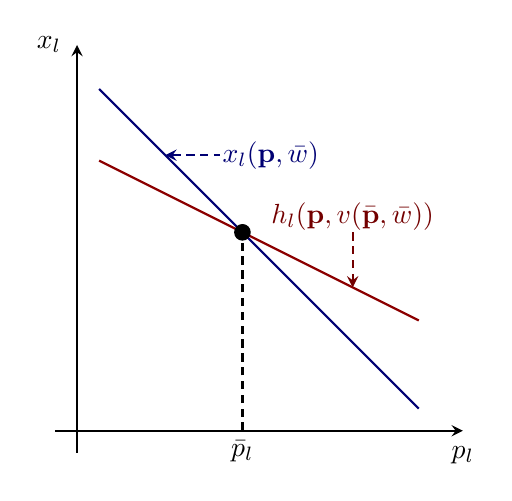
\begin{tikzpicture}[scale=1.4]
        % basics
        \draw [-stealth,color=black,thick] (-0.2,0) -- (3.5,0) node[below=2pt] {$p_l$};
        \draw [-stealth,color=black,thick] (0,-0.2) -- (0,3.5) node[left=2pt] {$x_l$};
        
        % walrasian
        \draw[domain=0.2:3.1, blue!45!black, thick, variable=\x] plot ({\x}, {3.3-\x});
        % hicksian
        \draw[domain=0.2:3.1, red!55!black, thick, variable=\x] plot ({\x}, {2.55-0.5*\x});
        % intersection: \bar{p}
        \filldraw[black] (1.5,1.8) circle (2pt); 
        % label
        \draw[densely dashed, thick, black] (1.5,0) node[below=0pt] {$\bar{p}_l$} (1.5,0) -- (1.5,1.8);
        
        % text
        \draw[-stealth,thick,densely dashed,red!45!black] (2.5,1.8) -- node[above=7pt] {$h_l(\mathbf{p},v(\bar{\mathbf{p}},\bar{w}))$} (2.5,1.3); % walrasian
        \draw[stealth-,thick,densely dashed,blue!45!black] (0.8,2.5) -- node[right=7pt] {$x_l(\mathbf{p},\bar{w})$} (1.3,2.5); % walrasian
    \end{tikzpicture}
    \caption*{Normal good}
\end{minipage}
\hfill
\begin{minipage}[b]{0.45\textwidth}
    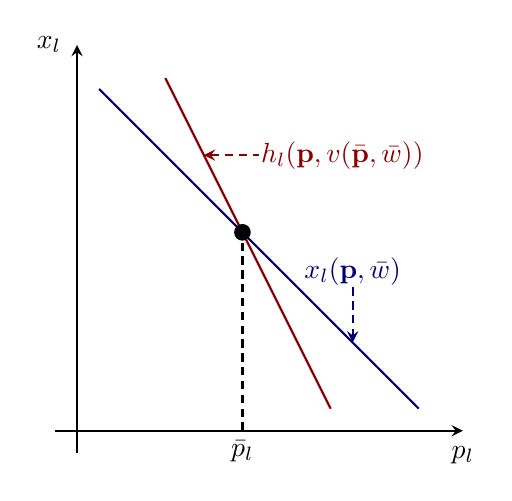
\begin{tikzpicture}[scale=1.4]
        % basics
        \draw [-stealth,color=black,thick] (-0.2,0) -- (3.5,0) node[below=2pt] {$p_l$};
        \draw [-stealth,color=black,thick] (0,-0.2) -- (0,3.5) node[left=2pt] {$x_l$};
        
        % walrasian
        \draw[domain=0.2:3.1, blue!45!black, thick, variable=\x] plot ({\x}, {3.3-\x});
        % hicksian
        \draw[domain=0.8:2.3, red!55!black, thick, variable=\x] plot ({\x}, {4.8-2*\x});
        % intersection: \bar{p}
        \filldraw[black] (1.5,1.8) circle (2pt); 
        % label
        \draw[densely dashed, thick, black] (1.5,0) node[below=0pt] {$\bar{p}_l$} (1.5,0) -- (1.5,1.8);
        
        % text
        \draw[-stealth,thick,densely dashed,blue!45!black] (2.5,1.3) -- node[above=7pt] {$x_l(\mathbf{p},\bar{w})$} (2.5,0.8); % walrasian
        \draw[stealth-,thick,densely dashed,red!55!black] (1.15,2.5) -- node[right=7pt] {$h_l(\mathbf{p},v(\bar{\mathbf{p}},\bar{w}))$} (1.65,2.5); % walrasian
    \end{tikzpicture}
    \caption*{Inferior good}
\end{minipage}
\end{figure}

When we focus on one good $l$, we have $\frac{\partial h_l(\bar{\mathbf{p}},\bar{u})}{\partial p_l} =\frac{\partial x_l(\bar{\mathbf{p}},\bar{w})}{\partial p_l} + \frac{\partial x_l (\bar{\mathbf{p}},\bar{w})}{\partial w}\cdot w_l(\bar{\mathbf{p}},\bar{w})$, the relationship between the Hicksian demand and the Walrasian demand becomes much more clear:
\begin{enumerate}
    \item[-] If good $l$ is normal good, then $\partial x_l (\bar{\mathbf{p}},\bar{w})/\partial w>0$, this means that if its price $p_l$ increases, Hicksian demand (with wealth increased accordingly to match the initial utility level $\bar{u}=v(\bar{\mathbf{p}},\bar{w})$) for good $l$ will decrease, but by a lower amount than the decrease of Walrasian demand (without wealth adjustment).
    \item[-] If good $l$ is inferior good, then $\partial x_l (\bar{\mathbf{p}},\bar{w})/\partial w<0$, the opposite logic follows. 
\end{enumerate}

Here, Slutsky (substitution) matrix appears once again. However, different from the choice-based, WARP-regulated demand, which requires the Slutsky matrix to be \textbf{negative semidefinite} and to satisfy $S(\mathbf{p},w)\mathbf{p}=0$ (see Thm.\ref{thm:slutksy_matrix_negativesemidef}), one extra condition is required for preference maximization: $S$ being \textbf{symmetric}.
The more essential distinction between these two approaches is that they adopt two different wealth compensation approaches: For an initial price-wealth pair $(\bar{\mathbf{p}},\bar{w})$ and its corresponding utility level $\bar{u}=u(\bar{x})$, and the price after change $\mathbf{p}'$:
\begin{enumerate}
    \item[-] Slutsky wealth compensation (Section\ref{chap2:sec2:ssec4}): wealth is adjusted from $\bar{w}$ to $w^S$ s.t. $\bar{x}$ could still be afforded, $w^S=\bar{x}\cdot \mathbf{p}'$, giving: $\Delta w_{\text{Slutsky}}=\mathbf{p}'\cdot x(\bar{\mathbf{p}},\bar{w})-\bar{w}$
    \item[-] Hicksian wealth compensation (this section): wealth is adjusted from from $\bar{w}$ to $w^H$ s.t. $\bar{u}$ could still be achieved, $v(\mathbf{p}',w^H)=\bar{u}$, giving: $\Delta w_{\text{Hicks}}=e(\mathbf{p}',\bar{u})-\bar{w}$
\end{enumerate}
The two compensation approaches are closely linked: $\Delta w_{\text{Hicks}}\leq \Delta w_{\text{Slutsky}}$, and since $\nabla_{\mathbf{p}}e(\bar{\mathbf{p}},\bar{u}) = h(\bar{\mathbf{p}},\bar{u})=x(\bar{\mathbf{p}},\bar{w})$, the equality holds \textbf{only} when the price change is a differential change ($\mathrm{d}p$):
\begin{align*}
    \Delta w_{\text{Slutsky}} &= \mathbf{p}'\cdot x(\bar{\mathbf{p}},\bar{w})-\bar{w} \\
    & \mathbf{p}'\cdot x(\bar{\mathbf{p}},\bar{w})-\bar{\mathbf{p}}\cdot x(\bar{\mathbf{p}},\bar{w})= x(\bar{\mathbf{p}},\bar{w})\cdot(\mathbf{p}'-\bar{\mathbf{p}}) \\
    & = \nabla_{\mathbf{p}}e(\bar{\mathbf{p}},\bar{u})\cdot(\mathbf{p}'-\bar{\mathbf{p}}) = e(\mathbf{p}',\bar{u})-e(\bar{\mathbf{p}},\bar{u})\\
    & = e(\mathbf{p}',\bar{u})-\bar{w} = \Delta w_{\text{Hicks}}
\end{align*}
the intuition is, for a very small change of price for good $l$, the total effect on the expenditure required to still achieve $\bar{u}$ is just the direct effect of the price change. But if the price change is not sufficiently small (discrete price changes), we would always have $\Delta w_{\text{Hicks}}< \Delta w_{\text{Slutsky}}$ (see Fig.\ref{fig:hicksian_slutsky_comp}).

\begin{figure}[ht]
    \centering
    \caption{Hicksian and Slutsky wealth compensation}
    \label{fig:hicksian_slutsky_comp}
    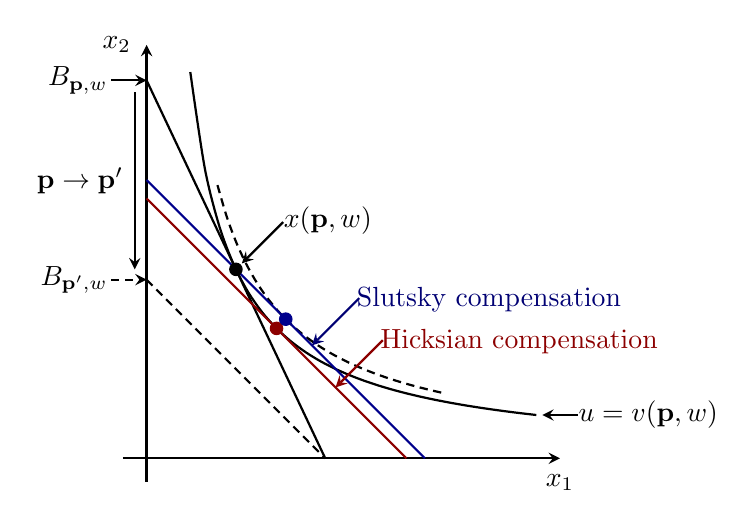
\begin{tikzpicture}[scale=1.5]
        % basics
        \draw [-stealth,color=black,thick] (-0.2,0) -- (3.5,0) node[below=2pt] {$x_1$};
        \draw [-stealth,color=black,thick] (0,-0.2) -- (0,3.5) node[left=2pt] {$x_2$};
        
        % utility and budget lines
        \draw[domain=0.37:3.3, smooth, thick, black, variable=\x] plot ({\x}, {1.1^2/\x}); % utility
        \draw[domain=0.6:2.5, smooth, thick, black, densely dashed, variable=\x] plot ({\x}, {(0.75625/2+1.1^2/(2*0.75625))^2/\x}); % slutsky utility
        \draw[domain=0:(4*1.1^2)/3.2, black, thick, variable=\x] plot ({\x}, {3.2-(3.2^2/(4*1.1^2))*\x}); % initial budget
        \draw[domain=0:(4*1.1^2)/3.2, densely dashed, black, thick, variable=\x] plot ({\x}, {(4*1.1^2)/3.2-\x}); % wealth-constant budget
        \draw[domain=0:2.2, red!55!black, thick, variable=\x] plot ({\x}, {2.2-\x}); % hicksian compensated budget
        \draw[domain=0:0.75625+1.1^2/0.75625, blue!55!black, thick, variable=\x] plot ({\x}, {0.75625+1.1^2/0.75625-\x}); % slutsky compensated budget
        
        % bundles
        \filldraw[black] (0.75625,1.1^2/0.75625) circle (1.5pt); % initial bundle
        \filldraw[red!55!black] (1.1,1.1) circle (1.5pt); % hicksian compensated bundle
        \filldraw[blue!55!black] (1.178125,1.178125) circle (1.5pt); % slutsky compensated bundle
        
        % texts and notes
        %% budget change
        \draw[-stealth,thick,black] (-0.3,3.2) -- node[left=4pt] {$B_{\mathbf{p},w}$} (0,3.2);
        
        \draw[-stealth,thick,densely dashed,black] (-0.3,1.5125) -- node[left=4pt] {$B_{\mathbf{p}',w}$} (0,1.5125);
        
        \draw[-stealth,thick] (-0.1,3.1) -- node[left=0.5pt] {$\mathbf{p}\rightarrow\mathbf{p}'$} (-0.1,1.6);
        
        %% utility
        \draw[stealth-,thick] (3.35,1.1^2/3.3) -- node[right=3pt] {$u=v(\mathbf{p},w)$} (3.65,1.1^2/3.3);
        
        
        %% bundles
        %%% initial bundle
        \draw[stealth-,thick,black] (0.75625+0.05,1.1^2/0.75625+0.05) -- node[right=4pt,yshift=8pt] {$x(\mathbf{p},w)$} (0.75625+0.4,1.1^2/0.75625+0.4);
        
        %%% Hicksian
        \draw[stealth-,thick,red!55!black] (1.6,0.6) -- node[right=4pt,yshift=8pt] {Hicksian compensation} (2,1);
         %%% Slutsky
        \draw[stealth-,thick,blue!45!black] (1.4,0.95625) -- node[right=4pt,yshift=8pt] {Slutsky compensation} (1.8,1.35625);
        
    \end{tikzpicture}
\end{figure}

\subsubsection*{$x(\mathbf{p},w)$ and $v(\mathbf{p},w)$}
Mirroring Thm.\ref{hdemand_and_exp}, we can link the Walrasian demand $x(\mathbf{p},w)$ and indirect utility function $v(\mathbf{p},w)$ through \textbf{Roy's identity}:
\begin{theorem}{Roy's identity}{roy_identity}
    With a continuous $u(\cdot)$ representing a locally nonsatiated, strictly convex $\succsim$, and an indirect utility function differentiable at $(\bar{\mathbf{p}},\bar{w})\gg 0$, the \myhl[blue]{Walrasian demand $x(\mathbf{p},w)$} is the (negative) derivative vector of $v(\mathbf{p},w)$ w.r.t. prices $\mathbf{p}$, \textbf{normalized} by marginal indirect utility of wealth:
    $$x(\bar{\mathbf{p}},\bar{w})=-\frac{1}{\nabla_w v(\bar{\mathbf{p}},\bar{w})}\nabla_{\mathbf{p}}v(\bar{\mathbf{p}},\bar{w})$$
    that is, $x_l(\bar{\mathbf{p}},\bar{w})=- \frac{\partial v(\bar{\mathbf{p}},\bar{w})/\partial p_l}{\partial v(\bar{\mathbf{p}},\bar{w})/\partial w},\forall l=1,\cdots,L$
\end{theorem}

Again, Roy's identity will be proved with 3 different approaches:
\begin{enumerate}
    \item[\textit{\textbf{Proof 1}}]: Let $\bar{u} = v(\bar{\mathbf{p}},\bar{w})$. Since $v(\mathbf{p},e(\mathbf{p},\bar{u}))=\bar{u},\forall \mathbf{p}$, differentiate the equation w.r.t. $\mathbf{p}$ and evaluating at $\mathbf{p}=\bar{\mathbf{p}}$, get
    \begin{align*}
        & \nabla_{\mathbf{p}} v(\bar{\mathbf{p}},e(\bar{\mathbf{p}},\bar{u})) + \frac{\partial v(\bar{\mathbf{p}},e(\bar{\mathbf{p}},\bar{u}))}{\partial w} \nabla_{\mathbf{p}}e(\bar{\mathbf{p}},\bar{u})=0 \\
        \xRightarrow{\text{Thm.\ref{thm:hdemand_and_exp}}} & \nabla_{\mathbf{p}} v(\bar{\mathbf{p}},e(\bar{\mathbf{p}},\bar{u})) + \frac{\partial v(\bar{\mathbf{p}},e(\bar{\mathbf{p}},\bar{u}))}{\partial w} h(\bar{\mathbf{p}},\bar{u})=0\\
        \xRightarrow[\bar{w}=e(\bar{\mathbf{p}},\bar{u})]{h(\bar{\mathbf{p}},\bar{u})=x(\bar{\mathbf{p}},\bar{w})} & \nabla_{\mathbf{p}} v(\bar{\mathbf{p}},\bar{w}) + \frac{\partial v(\bar{\mathbf{p}},\bar{w})}{\partial w} x(\bar{\mathbf{p}},\bar{w})=0\\
        \Rightarrow & x(\bar{\mathbf{p}},\bar{w})=-\frac{1}{\nabla_w v(\bar{\mathbf{p}},\bar{w})}\nabla_{\mathbf{p}}v(\bar{\mathbf{p}},\bar{w})
    \end{align*}

    \item[\textit{\textbf{Proof 2}}] FOC argument: assume $x(\mathbf{p},w)\gg 0$ and differentiable at $(\bar(\mathbf{p}),\bar{u})$, then by the chain rule, we have 
    \begin{align*}
        \left.\nabla_{\mathbf{p}}v(\mathbf{p},u)\right\vert_{(\bar{\mathbf{p}},\bar{w})}&=\nabla_{\mathbf{p}} u(x(\bar{\mathbf{p}},\bar{w}))=h(\mathbf{p},u)+\left[\mathbf{p}\cdot \mathrm{D}_{\mathbf{p}}h(\mathbf{p},u)\right]^T\\
        &=h(\mathbf{p},u)+\underbrace{\left[\underbrace{\lambda\nabla u(h(\mathbf{p},u))}_{\text{by FOC of EMP: }\mathbf{p}=\lambda\nabla u(h(\mathbf{p},u))} \cdot \mathrm{D}_{\mathbf{p}}h(\mathbf{p},u)\right]^T}_{\xRightarrow{\forall \mathbf{p},u(h(\mathbf{p},u))=u}=0}\\
        & = h(\mathbf{p},u)
    \end{align*}
    \item[\textit{\textbf{Proof 3}}] Envelope Theorem argument: assume $h(\mathbf{p},u)\gg 0$ and differentiable at $(\mathbf{p},u)$, then by the Envelope Theorem, we have 
    $$\nabla_{\mathbf{p}}e(\mathbf{p},u)=\nabla_{\mathbf{p}}(\mathbf{p}\cdot \mathbf{x}^{\text{optimal}})=\mathbf{x}^{\text{optimal}}=h(\mathbf{p},u)$$
\end{enumerate}

\section{Introducing Utility}\label{chap2:sec4}
%After examining the preference-based consumer theory, we have concluded that if a continuously differentiable demand function $x(\mathbf{p},w)$ is generated by rational preferences, this demand function must have
certain properties (see Thm.\ref{thm:properties_walrasian_demand}) and have a symmetric and negative semidefinite substitution matrix $S(\mathbf{p},w)$. In this section, we would examine the reverse:
if a demand function $x(\mathbf{p},w)$ has these properties, can it be rationalized by some preferences?

\subsection{Recover Preferences from Demand Functions}\label{chp2:sec4:ssec1}
The recovering $\succsim$ from $x(\mathbf{p},w)$ will be done in 2 steps:
\begin{enumerate}
    \item[-] \textbf{Step 1}: recover $e(\mathbf{p},u)$ from $x(\mathbf{p},w)$
    \item[-] \textbf{Step 2}: recover $\succsim$ from $e(\mathbf{p},u)$  
\end{enumerate}

\subsubsection*{Recover $e(\mathbf{p},u)$ from $x(\mathbf{p},w)$}
The first step is to recover $e(\mathbf{p},u)$ given a Walrasian demand function $x(\mathbf{p},w)$ that has the assumed properties: satisfies Walras' law, homogeneous of degree 0(see Thm.\ref{thm:properties_walrasian_demand}).
And, demand is assumed to be single-valued.

The recovering of $e(\mathbf{p},u)$ relies on the duality property $h(\mathbf{p},u)=x(\mathbf{p},e(\mathbf{p},u))$ and the proposition $h(\mathbf{p},u)=\nabla_{\mathbf{p}}e(\mathbf{p},u)$, combine these two, get:
$$
    \frac{\partial e(\mathbf{p})}{\partial p_i}=x_i(\mathbf{p},e(\mathbf{p})),\forall i=1,\cdots,L
$$
or, in a familiar form of expression
$$
\nabla_{\mathbf{p}}e(\mathbf{p})=x(\mathbf{p},e(\mathbf{p}))
$$

For this system of differential equations to have a solution, we must have $e(\mathbf{p})$ to be \textbf{twice continuously differentiable}, i.e., $e(\mathbf{p})$'s Hessian matrix is \myhl[blue]{\textbf{symmetric}}. Do the twice differentiation of $e(\mathbf{p})$:
\begin{align*}
    \mathrm{D}^2_{\mathbf{p}}e(\mathbf{p}) &= \mathrm{D}_{\mathbf{p}}x(\mathbf{p},e(\mathbf{p})) +\mathrm{D}_w x(\mathbf{p},e(\mathbf{p}))\cdot x(\mathbf{p},e(\mathbf{p}))^T\\
    & = S(\mathbf{p},e(\mathbf{p}))
\end{align*}
we actually get the Slutsky matrix again. Now we can conclude

\begin{enumerate}
    \item[-] $\nabla_{\mathbf{p}}e(\mathbf{p})=x(\mathbf{p},e(\mathbf{p}))$ has a solution $\Leftrightarrow$ the Slutsky matrix $S(\mathbf{p},w)$ being \textbf{symmetric}
    \begin{enumerate}
        \item[-] $\Rightarrow$: proved by the above equation, which requires the Slutsky matrix be the Hessian matrix of $e(\mathbf{p})$, which aligns with Thm.\ref{thm:prop_hick_pricederive}
        \item[-] $\Leftarrow$: by Frobenius theorem (see \hyperref[sssec:frobenius_theorem]{below} for details), the symmetry of $\nabla_{\mathbf{p}}$ at all points of its domain is equivalent to the existence of a solution 
    \end{enumerate}
    \item[-] the solution $e(\mathbf{p},u)$ has the properties of an expenditure function (Thm.\ref{thm:properties_expenditure_func}) $\Leftrightarrow$ the Slutsky matrix $S(\mathbf{p},w)$ being \textbf{negative semidefinite}
\end{enumerate}

Together, we have
\begin{proposition}{conditions of $S(\mathbf{p},w)$ to recover $e(\mathbf{p},u)$}{slutskycondition_recover}
    $S(\mathbf{p},w)$ being \myhl[blue]{\textbf{symmetric}} and \myhl[blue]{\textbf{negative semidefinite}} is the necessary and sufficient condition to recover $e(\mathbf{p},u)$
\end{proposition}

Prop.\ref{prop:slutskycondition_recover} is always true, and it can be linked to the discussion of WARP in the following way:
\begin{enumerate}
    \item[$L=2$] when there are only 2 goods, the Slutsky matrix is automatically symmetric, hence as long as the demand function $x(p_1,p_2,w)$ satisfies WARP (negative semidefiniteness guaranteed), $e(\mathbf{p},u)$ will be recovered:
    
    \begin{enumerate}
        \item[-] step 1: normalize $p_2=1$, pick an arbitrary price-wealth point $(p_1^0,1,w^0)$ and assign utility value $u^0$ to 
        \item[-] step 2: solve the differential equation 
        $$
        \frac{\mathrm{d}e(p_1)}{\mathrm{p_1}}=x_1(p_1,e(p_1))
        $$
        where $e(p_1)=e(p_1,1,u^0)$, $x_1(p_1,w)=x_1(p_1,1,w)$, with the initial condition $e(p_1^0)=w^0$
    \end{enumerate}
    Fig.\ref{fig:recover_exp_from_wal} illustrates the essence of this procedure intuitively: for any $(p_1,w)$, the demand function at the point $x_1(p_1,w)$ is the slope of some expenditure function, and for any given initial condition $(p_1^0,w^0)$, there will be an expenditure curve starts at it.
    \item[$L>2$] when there are more than 2 goods, WARP does not guarantee the symmetry of the Slutsky matrix, hence, symmetry condition must also be satisfied for the recovery of $e(\mathbf{p},u)$
\end{enumerate} 

\begin{figure}[ht]
    \centering
    \caption{Recover $e(\mathbf{p},u)$ from $x(\mathbf{p},w)$}
    \label{fig:recover_exp_from_wal}
    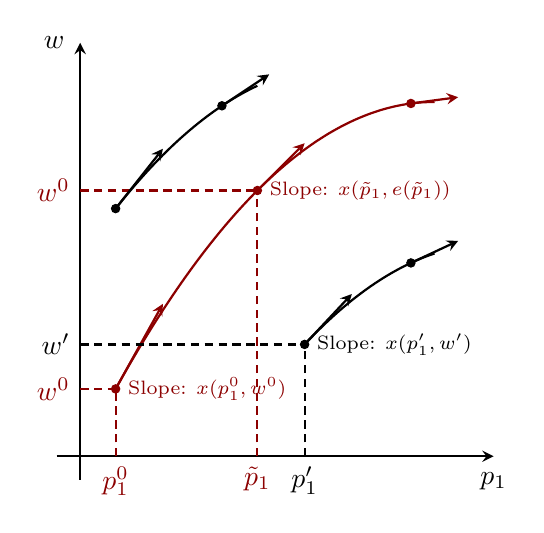
\begin{tikzpicture}[scale=1.5]
        % basics
        \draw [-stealth,color=black,thick] (-0.2,0) -- (3.5,0) node[below=2pt] {$p_1$};
        \draw [-stealth,color=black,thick] (0,-0.2) -- (0,3.5) node[left=2pt] {$w$};
        
        % correct e(p,u)
        \draw[domain=0.3:3, smooth, thick, red!55!black, variable=\x] plot ({\x}, {-1/3*(\x-3)^2+3});
        %% tangent 1
        \draw [-stealth,color=red!55!black,thick] (0.3,0.57) -- (0.7,1.29);
        \filldraw[red!55!black] (0.3,0.57) circle (1pt) node[right=1pt] {\scriptsize Slope: $x(p_1^0,w^0)$}; % initial bundle
        \draw[densely dashed,thick,red!55!black] (0.3,0) node[below] {$p_1^0$} --  (0.3,0.57);
        \draw[densely dashed,thick,red!55!black] (0,0.57) node[left] {$w^0$} -- (0.3,0.57);
        %% tangent 2
        \draw [-stealth,color=red!55!black,thick] (1.5,2.25) -- (1.9,2.65);
        \filldraw[red!55!black] (1.5,2.25) circle (1pt) node[right=1pt] {\scriptsize Slope: $x(\tilde{p}_1,e(\tilde{p}_1))$};
        \draw[densely dashed,thick,red!55!black] (1.5,0)  node[below] {$\tilde{p}_1$} -- (1.5,2.25);
        \draw[densely dashed,thick,red!55!black] (0,2.25) node[left] {$w^0$} -- (1.5,2.25);
        %% tangent 3
        \draw [-stealth,color=red!55!black,thick] (2.8,2.9867) -- (3.2,3.04);
        \filldraw[red!55!black] (2.8,2.9867) circle (1pt);
        
        % alternate 1
        \draw[domain=1.9:3, smooth, thick, black, variable=\x] plot ({\x}, {-1/3*(\x-3.5)^2+1.8});
        %% tangent a1
        \draw [-stealth,color=black,thick] (1.9,0.9467) -- (2.3,1.37337);
        \filldraw[black] (1.9,0.9467) circle (1pt) node[right=1pt] {\scriptsize Slope: $x(p'_1,w')$}; % initial bundle
        \draw[densely dashed,thick,black] (1.9,0) node[below] {$p'_1$} --  (1.9,0.9467);
        \draw[densely dashed,thick,black] (0,0.9467) node[left] {$w'$} -- (1.9,0.9467);
        %% tangent a2
        \draw [-stealth,color=black,thick] (2.8,1.6367) -- (3.2,1.82337);
        \filldraw[black] (2.8,1.6367) circle (1pt);
        
        % alternate 2
        \draw[domain=0.3:1.5, smooth, thick, black, variable=\x] plot ({\x}, {-1/3*(\x-2.2)^2+3.3});
        %% tangent b1
        \draw [-stealth,color=black,thick] (0.3,2.0967) -- (0.7,2.6033);
        \filldraw[black] (0.3,2.0967) circle (1pt);
        %% tangent b2
        \draw [-stealth,color=black,thick] (1.2,2.967) -- (1.6,3.233);
        \filldraw[black] (1.2,2.967) circle (1pt);
        
    \end{tikzpicture}
\end{figure}

\subsubsection*{Recover $\succsim$ from $e(\mathbf{p},u)$}
The second step is to recover $\succsim$ given an expenditure function $e(\mathbf{p},u)$ that has the assumed properties: continuous, strictly increasing in $u$, non-decreasing, homogeneous of degree 1, and concave in $\mathbf{p}$ (see Thm.\ref{thm:properties_expenditure_func}).
Since demand is single-valued, $e(\mathbf{p},u)$ is also differentiable.

Here, let $V_u\subset \mathbb{R}^L$  be an at-least-as-good-as set for each utility level $u$ s.t. $e(\mathbf{p},u)$ is the minimal expenditure required for a bundle in $V_u$ at price $\mathbf{p}\gg  0$, i.e. 
$$
e(\mathbf{p},u)=\min_{\mathbf{x}\geq 0}\mathbf{p}\cdot \mathbf{x}\ \text{ s.t. }\mathbf{x}\in V_u
$$

Intuitively, the set $V_u = \left\{ \mathbf{x} \in\mathbb{R}^L_+\mid \mathbf{p}\cdot \mathbf{x}\geq e(\mathbf{p},u),\forall \mathbf{p}\gg 0 \right\}$ satisfies the requirement, that is 
\begin{proposition}{At-least-as-good-as set $V_u$}{atleastasgoodasset_exp}
    For $e(\mathbf{p},u)$ that is strictly increasing in $u$, continuous, non-decreasing, homogeneous of degree 1, concave and differentiable in $\mathbf{p}$, then $\forall u$, $e(\mathbf{p},u)$ is the expenditure function associated with the at-least-as-good-as set
    $$
    V_u = \left\{ \mathbf{x}\in\mathbb{R}^L_+\mid \mathbf{p}\cdot\mathbf{x}\geq e(\mathbf{p},u),\forall \mathbf{p}\gg 0 \right\}
    $$
    i.e. $e(\mathbf{p},u)=\min\left\{ \mathbf{p}\cdot \mathbf{x}\mid \mathbf{x}\in V_u \right\},\forall \mathbf{p}\gg 0$.
\end{proposition}

\textbf{Proof}: Immediately by definitions, $e(\mathbf{p},u)\leq \min\left\{\mathbf{p}\cdot\mathbf{x}\mid \mathbf{x}\in V_n\right\}$. Next, prove $e(\mathbf{p},u)\geq \min\left\{\mathbf{p}\cdot\mathbf{x}\mid \mathbf{x}\in V_n\right\}$: since $e(\mathbf{p},u)$ is concave in $\mathbf{p}$, we have
$$
e(\mathbf{p}',u)\leq e(\mathbf{p},u)+\nabla_{\mathbf{p}}e(\mathbf{p},u)\cdot(\mathbf{p}'-\mathbf{p}),\forall \mathbf{p},\mathbf{p}'
$$
since $e(\mathbf{p},u)$ is homogeneous of degree 1, by Euler's formula, $e(\mathbf{p},u)=\mathbf{p}\cdot\nabla_{\mathbf{p}}e(\mathbf{p},u)$, hence $e(\mathbf{p}',u)\leq \mathbf{p}'\cdot \nabla_{\mathbf{p}}e(\mathbf{p},u),\forall \mathbf{p}'$, plus the fact that $\nabla_{\mathbf{p}(\mathbf{p},u)}\geq 0$, gives that $\nabla_{\mathbf{p}(\mathbf{p},u)}\in V_u$.
By the definition of the at-least-as-good-as set $V_u$, we have $\min\left\{\mathbf{p}\cdot\mathbf{x}\mid \mathbf{x}\in V_u\right\}\leq \mathbf{p}\cdot \nabla_{\mathbf{p}(\mathbf{p},u)}=e(\mathbf{p},u)$. The proof is finished.

With Prop.\ref{prop:atleastasgoodasset_exp}, we can find a set of $V_u$ for each level of $u$, and since $\partial e(\mathbf{p},u)/\partial u>0$, we have $u'>u\Rightarrow V_{u'}\subset V_u$. Each $V_u$ is closed, convex, and bounded below, hence these at-least-as-good-as sets can define a 
preference $\succsim$ (represented by utility levels $u$) that has $e(\mathbf{p},u)$ as its expenditure function (see Fig.\ref{fig:recover_pref_from_exp}).

\begin{figure}[ht]
    \centering
    \caption{Recover $\succsim$ from $e(\mathbf{p},u)$}
    \label{fig:recover_pref_from_exp}
    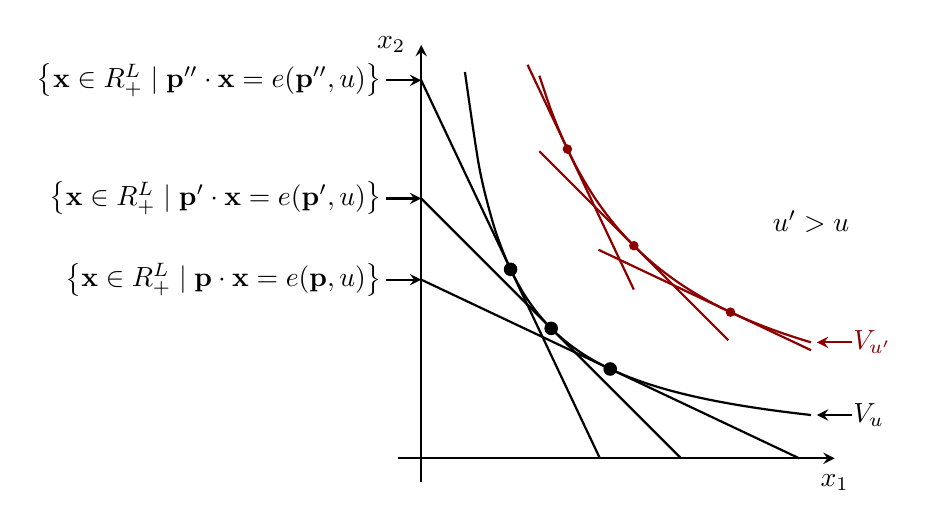
\begin{tikzpicture}[scale=1.5]
        % basics
        \draw [-stealth,color=black,thick] (-0.2,0) -- (3.5,0) node[below=2pt] {$x_1$};
        \draw [-stealth,color=black,thick] (0,-0.2) -- (0,3.5) node[left=2pt] {$x_2$};
        
        % utility and budget lines
        \draw[domain=0.37:3.3, smooth, thick, black, variable=\x] plot ({\x}, {1.1^2/\x}); % utility
        
        \draw[domain=1:3.3, smooth, thick, red!55!black, variable=\x] plot ({\x}, {1.8^2/\x}); % utility'
        
        \draw[domain=0:(4*1.1^2)/3.2, black, thick, variable=\x] plot ({\x}, {3.2-(3.2^2/(4*1.1^2))*\x}); % budget 1
        \draw[domain=0:2.2,black, thick, variable=\x] plot ({\x}, {2.2-\x}); % budget 2
        \draw[domain=0:3.2, black, thick, variable=\x] plot ({\x}, {((4*1.1^2)/3.2)-((4*1.1^2)/3.2^2)*\x}); % budget 3
        
        \draw[domain=0.9:1.8, red!55!black, thick, variable=\x] plot ({\x}, {5.23636-(3.2^2/(4*1.1^2))*\x}); % budget 1'
        \draw[domain=1:2.6,red!55!black, thick, variable=\x] plot ({\x}, {3.6-\x}); % budget 2'
        \draw[domain=1.5:3.3, red!55!black, thick, variable=\x] plot ({\x}, {2.475-((4*1.1^2)/3.2^2)*\x}); % budget 3'
        
        
        
        % bundles
        \filldraw[black] (0.75625,1.1^2/0.75625) circle (1.5pt); % bundle 1
        \filldraw[black] (1.1,1.1) circle (1.5pt); %  bundle 2
        \filldraw[black] (1.1^2/0.75625,0.75625) circle (1.5pt); % bundle 3
         % bundles
        \filldraw[red!55!black] (1.2375,1.8^2/1.2375) circle (1pt); % bundle 1'
        \filldraw[red!55!black] (1.8,1.8) circle (1pt); %  bundle 2'
        \filldraw[red!55!black] (1.8^2/1.2375,1.2375) circle (1pt); % bundle 3'
        
        %% utility
        \draw[stealth-,thick] (3.35,1.1^2/3.3) -- node[right=3pt] {$V_u$} (3.65,1.1^2/3.3);
        \draw[stealth-,thick,red!55!black] (3.35,1.8^2/3.3) -- node[right=3pt] {$V_{u'}$} (3.65,1.8^2/3.3);
        
        % texts and notes
        %% budget change
        \draw[-stealth,thick,black] (-0.3,3.2) -- node[left=4pt] {$\left\{\mathbf{x}\in\mathbb{R}^L_+\mid \mathbf{p}''\cdot\mathbf{x}=e(\mathbf{p}'',u) \right\}$} (0,3.2);
        \draw[-stealth,thick,black] (-0.3,2.2) -- node[left=4pt] {$\left\{\mathbf{x}\in\mathbb{R}^L_+\mid \mathbf{p}'\cdot\mathbf{x}=e(\mathbf{p}',u) \right\}$} (0,2.2);
        \draw[-stealth,thick,black] (-0.3,1.5125) -- node[left=4pt] {$\left\{\mathbf{x}\in\mathbb{R}^L_+\mid \mathbf{p}\cdot\mathbf{x}=e(\mathbf{p},u) \right\}$} (0,1.5125);
        
        \node at (3.3,2) {$u'>u$};
        
    \end{tikzpicture}
\end{figure}

This conclusion can be extended to the case that the underlying preferences of $e(\mathbf{p},u)$ is \textbf{non-convex}. A non-convex $\succsim$ will generate a non-convex 
at-least-as-good-as set, as shown in Fig.\ref{fig:recover_pref_from_exp_nonconvex}.

\begin{figure}[ht]
    \centering
    \caption{Recover non-convex $\succsim$ from $e(\mathbf{p},u)$}
    \label{fig:recover_pref_from_exp_nonconvex}
    \begin{tikzpicture}[scale=1.5]
        % basics
        \draw [-stealth,color=black,thick] (-0.2,0) -- (3.5,0) node[below=2pt] {$x_1$};
        \draw [-stealth,color=black,thick] (0,-0.2) -- (0,3.5) node[left=2pt] {$x_2$};
        
        \draw [thick,red!55!black,tangent=0.9] (0.37,3.3) .. controls (0.5,2.2) and (0.6,1.5) .. (0.8,1.5);
        \draw [black, thick, use tangent] (-1,0) -- (2,0);
        
        \draw [thick,red!55!black,tangent=0.1] (1.5,0.8) .. controls (1.5,0.6) and (2.2,0.5) .. (3.3,0.37);
        \draw [black, thick, use tangent] (-2,0) -- (1,0);
        
        %non-convex part
        \draw [thick,dashed,red!55!black] (0.8,1.5).. controls (1.4,1.4).. (1.5,0.8);
        \draw[domain=0.2:2.05,red!55!black, thick, variable=\x] plot ({\x}, {2.25-\x});
        
        % notes
        %%% actual
        \draw[stealth-,dashed, thick,red!55!black] (1.36,1.36) -- node[right=5pt,yshift=10pt,align=left] {Boundary of \textbf{actual} \\ at-least-as-good-as set} (1.7,1.7);
         %%% Slutsky
        \draw[-stealth,thick,black] (1.125-0.4,1.125-0.4) -- node[left=5pt,yshift=-10pt] {Boundary of $V_u$} (1.12,1.12);
        %%% price-utility
        \draw[stealth-,thick,black] (2.05,0.2) -- node[right=5pt] {\scriptsize $\left\{\mathbf{x}\in\mathbb{R}^L_+\mid \mathbf{p}^*\cdot\mathbf{x}=e(\mathbf{p}^*,u^*)\right\}$} (2.4,0.2);
    \end{tikzpicture}
\end{figure}

For this non-convex at-least-as-good-as set, we can always find its convex hull (the solid line) that also generates the
expenditure function $e(\mathbf{p}),u)$. 
Here we have the correspondence between the differentiability of $e(\mathbf{p},u)$ and the , for a specific price-utility pair $(\mathbf{p}^*,u^*)$, there would be more than one expenditure minimizers, and at this price-utility pair $(\mathbf{p}^*,u^*)$,
 the generated $e(\mathbf{p},u)$ would \textbf{NOT} be differentiable. This can be summarized as:
$$
e(\mathbf{p},u) \text{ is differentiable}\Rightarrow \succsim \text{ is convex}
$$

With the two steps, $\succsim$ can be recovered from demand function $x(\mathbf{p},w)$ through expenditure function $e(\mathbf{p},u)$. This problem, especially the problem of recovering $e(\mathbf{p},u)$ from $x(\mathbf{p},u)$, which involves the differential equation $h(\mathbf{p},u)=\nabla_{\mathbf{p}}e(\mathbf{p},u)$, is the \textbf{integrability} problem.

\subsection{Discussion on integrability}\label{sssec:integrability}
The discussion on recovering preferences from demand functions is based on Hurwicz and Uzawa's work, to summarize, we have
\begin{enumerate}
    \item[-] \myhl[blue!45!black]{\textbf{(B)}}: \underline{\textbf{budget}} exhaustion: $\mathbf{p}\cdot x(\mathbf{p},w)=w$
    \item[-] \myhl[blue!45!black]{\textbf{(D)}}: the demand function $x(\mathbf{p},w)$ is \underline{\textbf{differentiable}} everywhere
    \item[-] \myhl[blue!45!black]{\textbf{(S)}}: the Slutsky matrix $S(\mathbf{p},w)$ is \underline{\textbf{symmetric}}
    \item[-] \myhl[blue!45!black]{\textbf{(NSD)}}: the Slutsky matrix $S(\mathbf{p},w)$ is \underline{\textbf{negative semidefinite}}
    \item[-] \myhl[blue!45!black]{\textbf{(IB)}}: the demand function $x(\mathbf{p},w)$ satisfies the \underline{\textbf{boundedness}} condition: $$ \left\vert \frac{\partial x_i(\mathbf{p},w)}{\partial w} \right\vert \leq M < \infty, \forall i=1,\cdots,n,\forall m\geq 0 $$
\end{enumerate}

These assumptions are required for the process of recovering preferences from demand functions discussed above: If all 5 of Hurwicz-Uzawa assumptions are satisfied, then $\exists u$ s.t. $\forall (\mathbf{p},w)$, $x(\mathbf{p},w)$ is the \myhl[blue!45!black]{\textbf{unique}} maximizer of $u$ over the budget set $\left\{ \mathbf{x}: \mathbf{p}\cdot \mathbf{x}\leq w\right\}$.

To integrate from demand $x(\mathbf{p},w)$ to a utility function, it is sufficient to integrate from $x(\mathbf{p},w)$ to the indirect utility function $v(\mathbf{p},w)$, then $x(\cdot)$ and $v(\cdot)$ must satisfy the Hotelling's lemma:
$$
-\frac{v_{\mathbf{p}}(\mathbf{p},w)}{v_{w}(\mathbf{p},w)} = \mathbf{x}(\mathbf{p},w)
$$
From this, we have two separate aspects to understand integrability: 
\begin{enumerate}
    \item[-] \textit{mathematical} integrability: the existence of $v(\cdot)$ to satisfy the differential equation above.
    \item[-] \textit{economic} integrability: $v(\cdot)$ should be a well-behaved indirect utility function as well, corresponding to a direct utility function.
\end{enumerate}

This result is quite general and is one of the fundamental results, some recent work seeks to extend it to reflect the nuance of empirical observations. I have searched some papers on this topic and will briefly discussed the results here. For a rather thorough discussion on the development of this topic, see \citet*{hands2006integrability}.

\subsubsection*{Incomplete systems of demand functions}
Hurwicz and Uzawa's result is theoretically exhaustive, in the sense that as long as the 5 integrability conditions are satisfied, with suitable regularity conditions assumed, \textbf{any} set of demand functions can be retionalized by some utility function. \cite{epstein1982integrability} discussed the problem of incomplete sets of demand functions.

Consider the utility maximization problem of a consumer:
$$
\max_{\mathbf{x},\mathbf{y},z} \left\{ u(\mathbf{x},\mathbf{y},z)\mid \mathbf{p}\cdot\mathbf{x}+\mathbf{q}\cdot \mathbf{y} + z =w, \mathbf{x},\mathbf{y},z\geq 0 \right\}
$$
where $\mathbf{x}$ is the set of \textbf{observed} demands (priced at $\mathbf{p}$), and $\left(\mathbf{y},z\right)$ is the unobservable set of demands (priced as $(\mathbf{q},1)$, z is the numeraire). If the observed $\mathbf{x}$ is part of the solution to the utility maximization problem, it will have some of the properties (notably symmetry and negative semi-definiteness) like that for complete demand systems. However, Hurwicz-Uzawa integrability conditions are \textbf{not enough} to guarantee the
existence of a utility function for incomplete demand functions. Instead, they proposed that if the observed demand function $\mathbf{x}(w,\mathbf{p},\mathbf{q}): \Omega^{1+n+m}\rightarrow \Omega^n$\sidenotes{$\leftarrow$ $n$ observed, $m+1$ unobserved} such that 
\begin{enumerate}
    \item[1.] budget binding: $\forall (w,\mathbf{p},\mathbf{q})$, $\mathbf{p}x(w,\mathbf{p},\mathbf{q})<w,x(w,\mathbf{p},\mathbf{q})>0$
    \item[2.] $x^i(w,\mathbf{p},\mathbf{q})$ is \textbf{twice continuously differentiable} for all $i$
    \item[3.] The $n\times n$ matrix $x_{\mathbf{p}}(w,\mathbf{p},\mathbf{q}) + x(w,\mathbf{p},\mathbf{q})\cdot x_w (w,\mathbf{p},\mathbf{q})$ (Slutsky matrix for observed demands) is \textbf{negative \myhl[red!55!black]{definite}}
\end{enumerate}
Then there exists a \textbf{continuous, non-decreasing and \myhl[red!55!black]{quasiconcave}} utility function $u$ and a \myhl[red!55!black]{\textbf{neighborhood}} $N$ of $(w^0,\mathbf{p}^0,\mathbf{q}^0)$ s.t. $\forall (w,\mathbf{p},\mathbf{q})\in N$, $x(w,\mathbf{p},\mathbf{q})$ is the unique solver of the aforementioned utility maximizing problem.

The key argument of \cite{epstein1982integrability} is the \textbf{negative \myhl[red!55!black]{definiteness}} of the Slutsky matrix of the observed demands, and one thing very important about this result is that it is a \myhl[red!55!black]{\textbf{local}} result. The proof is skipped here, but duality also plays a crucial role as before.

To extend this local result to possible global results, some extra conditions must be met. \citet*{epstein1982integrability} proposed that if $x_{\mathbf{q}}(w,\mathbf{p},\mathbf{q})=0$, the 3 conditions will guarantee the glocal integrability of $x(\cdot)$, that is, observed demands (the first $n$ goods) are independent of the prices of the remaining $(m+1)$ goods (demands unobserved). This result is quite intuitive: consider the case of $n=1$, that is, the demand of only one good is observed. If other (normalized) prices $\mathbf{q}$ are constant, then this problem can fit into a two-good framework and the standard integrability results apply. \citet*{epstein1982integrability} also proposed several classes of demand functions $x(\cdot)$ that have global integrability (see Table 1 on Page 419 of the paper for details).

\citet*{lafrance1989dual} generalized \citeauthor*{epstein1982integrability}'s result by employing an arbitrary price index for the goods of which the demand is unobserved: $\pi(\mathbf{q})$. This deflator function $\pi(\mathbf{q})$\footnote{some examples are: $\pi(\mathbf{q})\equiv q_1$, $\pi(\mathbf{q})\equiv \sum^m_{j=1}\alpha_jq_j$, $\pi(\mathbf{q})\equiv \prod^m_{j=1}q_j^{\alpha_j}$, where $\sum^m_{j=1}\alpha_j=1,\alpha_j\geq 0$.} is used to normalize $\mathbf{p}$ and $w$. In addition to the 3 conditions of \citeauthor*{epstein1982integrability}, \citeauthor*{lafrance1989dual} gave a condition on $\pi(\mathbf{q})$ to guarantee the \myhl[blue!45!black]{\textbf{global}} integrability: $\exists \pi:\mathbb{R}^m_{++}\rightarrow \mathbb{R}_+$ s.t. $\pi\in C^2$ is \textbf{increasing}, \textbf{homogeneous of degree 1}, \textbf{concave in }$\mathbf{q}$ and $x(w,\mathbf{p},\mathbf{q})=\tilde{x}\left(\frac{1}{\pi(\mathbf{q})}\cdot w,\frac{1}{\pi(\mathbf{q})}\cdot\mathbf{p}\right)$. This condition requires that the observed demands depend upon the prices of other goods \textbf{only} through a price index that deflates the prices of the observed goods and total expenditure. 

However, this condition depends on the separability of $\mathbf{q}$ from $(\mathbf{p},w)$ in the indirect utility function: $v(w,\mathbf{p},\mathbf{q})\equiv \varphi\left(\frac{w}{\pi(\mathbf{q})},\frac{w}{\pi(\mathbf{q})}\right)$ and in the expediture function $e(u,\mathbf{p},\mathbf{q})\equiv \pi(\mathbf{q})\epsilon\left(\frac{\mathbf{p}}{\pi(\mathbf{q})},u\right)$. This is equivalent to a homothetically separable utility function: $u(\mathbf{x},\mathbf{y})\equiv \bar{u}\left(\mathbf{x},f(\mathbf{y})\right)$\sidenotes{$\leftarrow$ here the notation is modified for convenience, $\mathbf{x}$ is still the vector of observed demands, $\mathbf{y}$ is the vector of unobserved demands}, where $f(\cdot)$ is homogeneous of degree 1. Obviously, this is a very restrictive condition. Therefore, \citeauthor*{lafrance1989dual} introduced the concept of \myhl[red!55!black]{\textbf{weak integrability}}: If $\forall (w,\mathbf{p},\mathbf{q})$, there is a function $\nu:\mathbb{R}^{n+m+1}_{++}\rightarrow \mathbb{R}$ that is \textbf{continuous, increasing and quasiconcave} in $(\mathbf{x},s)$ where $\mathbf{x} = x(w,\mathbf{p},\mathbf{q})$ and $s=\sigma(w,\mathbf{p},\mathbf{q})\equiv y-\mathbf{p}\cdot\mathbf{x}$\footnote{Here, $\mathbf{x}$ is still the observed demands, and $s$ is the expenditure on all other goods: $s\equiv \mathbf{q}\cdot \mathbf{z}$} solves the maximization problem:
$$
\max_{\mathbf{x},s}\left\{ \nu(\mathbf{x},s,\mathbf{q}) \mid \mathbf{p}\cdot\mathbf{x}+s\leq w, \mathbf{x}\geq 0,s>0 \right\}
$$
and the duality is established in the same way as the complete demand system: \textbf{weak} integrability is equivalent to the existence of an expenditure function $e(\mathbf{p},\mathbf{q},u)$ that is increasing and concave in $\mathbf{p}$, homogeneous of degree 1 in $(\mathbf{p},\mathbf{q})$, and satisfies 
$$
\mathbf{p}\cdot x(e(\mathbf{p},\mathbf{q},u),\mathbf{p},\mathbf{q}) + \sigma(e(\mathbf{p},\mathbf{q},w),\mathbf{p},\mathbf{q})\equiv e(\mathbf{p},\mathbf{q},u)
$$
and Hotelling's lemma. 

\citeauthor*{lafrance1989dual} proved that the following conditions need to be satisfied to achieve (global) weak integrability:
\begin{enumerate}
    \item[-] $x(\cdot)\in C^2$, homogeneous of degree 0 in $(w,\mathbf{p},\mathbf{q})$
    \item[-] $x(w,\mathbf{p},\mathbf{q})\geq 0$, $\mathbf{p}\cdot x(w,\mathbf{p},\mathbf{q})<w$ (positive and not budget-exhausting)
    \item[-] Slutsky matrix $S$ is \textbf{symmetric, negative \myhl[red!55!black]{semidefinite}}
\end{enumerate} 
These conditions are pretty much the same as the integrability condition for complete demand systems. In addition,
\begin{enumerate}
    \item[-] $e(\cdot)\in C^3$ in $\mathbf{p}$: extra degree of differentiability to guarantee $x(\cdot)\in C^2$
    \item[-] $\forall (w,\mathbf{p},\mathbf{q})$, $s$ satisfies $\frac{\partial s_{ij}}{\partial w}=\frac{\partial s_{ji}}{\partial w}$ and $\frac{\partial s_{ij}}{\partial p_k}=\frac{\partial s_{ji}}{\partial p_k},\forall i,j,k=1,\cdots, n$: given by the symmetry of Slutsky matrix.
\end{enumerate}
These conditions are much easier to satisfy and verify empircally. \citeauthor*{lafrance1989dual} also discussed welfare implications of this result.

\subsubsection*{Linear and quasi-linear integrability}

\citet*{amir2017microeconomic} surveys the microfoundation of \textbf{linear demand} and discussed the integrability of it. Linear demand is the solution to the quadratic utility maximization problem, 

Consider the numeraire as additively separable, the UMP is then:
\begin{align*}
    \max & U(\mathbf{x})+y & \text{s.t. }&\mathbf{p}\cdot\mathbf{x}+y\leq w
\end{align*}
with Walrasian demand $(\mathbf{x}^*,y^*)$ as its solution. 

Its dual problem (EMP) is 
\begin{align*}
    \min & \mathbf{p}\cdot\mathbf{x}+y & \text{s.t. }U(\mathbf{x})+y&\geq u
\end{align*}
with Hicksian demand $(\mathbf{x}^h,y^h)$ as its solution.
\citeauthor*{amir2017microeconomic} showed that under quasi-linear utility, both the Walrasian demand and the Hicksian demand satisfy the Law of Demand\footnote{For the Hicksian demand: by convex analysis, $\frac{\partial e(\mathbf{p},u)}{\partial p_i}=x^h_i$ (which is just Shepard's Lemma). For Walrasian, since utility is quasi-linear in the numeraire, there are no income effects.}. Here, the result does NOT reply on the classic assumption that the utility function is quasi-concave.

Now we look at the case of quadratic utility: $U(x)=\mathbf{a}'\mathbf{x}-\frac{1}{2}\mathbf{x}'\mathbf{B}\mathbf{x}$, where $\mathbf{a}\in \mathbb{R}^n_{++}$, $\mathbf{B}$ is an $n\times n$ matrix, normalized to be symmetric and have all its diagonal entries equal to 1. Then the utility maximization problem is
$$
\max \left\{ \mathbf{a}'\mathbf{x}-\frac{1}{2}\mathbf{x}'\mathbf{B}\mathbf{x}+y \right\}\ \text{s.t. }\mathbf{p}'\mathbf{x}+y=w
$$
Here, the demand function is linear \sidenotes{The demand function is actually an \textbf{affine} function whenever positive and 0 otherwise, to be precise.}, for the consumer's problem to have an \myhl[blue!45!black]{\textbf{interior}} solution and preserve the \myhl[blue!45!black]{\textbf{linear}} nature of the resulting demand function, we need:
\begin{align*}
    \mathbf{B}^{-1}(\mathbf{a}-\mathbf{p})&>0 & \mathbf{p}'\mathbf{B}^{-1}(\mathbf{a}-\mathbf{p})\leq w
\end{align*}
so the essential condition here is $\mathbf{B}$ is \myhl[red!55!black]{\textbf{inversible}}, i.e., $U$ is \textbf{strictly} concave. This gives a significant result: $\mathbf{B}$ is positive definite, then the inverse demand and the direct demand satisfy the \myhl[blue!45!black]{\textbf{strict Law of Demand}}:
$$
\left[ U(\mathbf{x}) - U(\mathbf{x}') \right]\cdot \left( \mathbf{x}-\mathbf{x}' \right) <0,\ \forall \mathbf{x},\mathbf{x}'\in \mathbb{R}^n_{+}
$$
let $\mathbf{M}=\mathbf{B}^{-1}$, then $\exists$ a continuous utility $U:\mathbb{R}^n_{+}\rightarrow \mathbb{R}$ s.t. the linear demand function $D(\mathbf{p})=\mathbf{d}-\mathbf{Mp}$ with $d_i\geq 0,\forall i$ can be obtained by solving
$$
\max\left\{U(\mathbf{x}+y)\right\}\ \text{s.t.}\mathbf{p'x}+y\leq w
$$
since $\mathbf{M}=\mathbf{B}^{-1}$, it is symmetric and positive definite as well.
Using this result, \citeauthor*{amir2017microeconomic} discussed a widely used utility specification characterized by a \textbf{fully symmetric} substitution/complementarity matrix
$$
\mathbf{B}=\begin{bmatrix}
    1 & \gamma &\cdots &\gamma\\
    \gamma & 1 & \ddots & \vdots\\
    \vdots & \ddots & \ddots & \gamma\\
    \gamma & \cdots & \gamma & 1
\end{bmatrix}
$$
for it to be strictly concave, $\gamma\in \left(-\frac{1}{n-1},1\right)$. 
The main message of this result is that any linear demand that maximizes the utility of a representative consumer necessarily possesses strong regularity properties.

\citet*{nocke2017quasi} extended the quasi-linear integrability for all continuous demand systems that do not depend on income, their approach is:
\begin{enumerate}
    \item[1.] show the existense of an indirect subutility function
    \item[2.] construct a direct quasi-linear utility function with duality theory
    \item[3.] show that: quasi-linear integrability $\Leftrightarrow$ the demand system being a conversative vector field $\Leftrightarrow$ 
\end{enumerate}

\subsection{Frobenius theorem}\label{sssec:frobenius_theorem}
The Frobenius theorem is one of the fundamental theorems in differential topology. It is the foundation for the disucssion of the integrability problem, which I think it's worth spending some time understanding the basics. The discussion below is by no means thorough or rigorous\footnote{For more math, check \cite{sternberg1999lectures}, \cite{warner1983foundations}, \cite{mccleary2013geometry}}, but my own interpretation of this topic.

\subsubsection*{Frobenius theorem (vector field version)}
Frobenius theorem can be illustrated with the language of vector fields, for which some basic definitions need to be introduced.

\begin{definition}{Basic definitions of differntial geometry}{def}
    \begin{enumerate}
        \item[1] \textbf{smooth differentiable manifold} $M$ is a collection of \textbf{open} sets $U_{\alpha}\subset M$ and a collection of homeomorphisms $\varphi_{\alpha}:U_{\alpha}\rightarrow\mathbb{R}^N$ that satisfies
        \begin{enumerate}
            \item[-] $\bigcup_{\alpha}U_{\alpha}=M$ {(\color{red!55!black}$U_{\alpha}$\textit{ are the coordinate neighborhoods})}
            \item[-] when $U_{\alpha}\cap U_{\beta}\neq \varnothing$, the mapping $\varphi_{\alpha}\circ \varphi_{\beta}^{-1}:\varphi_{\beta}(U_{\alpha}\cap U_{\beta})\rightarrow \varphi_{\alpha}(U_{\alpha}\cap U_{\beta})$ is $C^{\infty}$ {\color{red!55!black}($M$ has a countable base)}
        \end{enumerate}
        \item[2] \textbf{coordinates}: define the $k-$th coordinate projection by $r^k\left(x^1,\cdots,x^N\right)=x^k$, then the coordinates on $M$ is 
        $$
        x^k = r^k\circ \varphi_{\alpha}: U_{\alpha}\rightarrow \mathbb{R}
        $$
        if $x\in U_{\alpha}$, $x$ is uniquely determined by its coordinates $\left(x^1(x),\cdots,x^m(x)\right)$
        \item[3] \textbf{tangent vectors} for a curve $\gamma:(-a,a)\rightarrow M$, its tangent vector $X$ maps a smooth function $f:M\rightarrow \mathbb{R}$ to its \underline{\textbf{directional derivative} $X(f)$} \footnote{derivative of $f$ in the direction $X$}. At a point $x\in M$, the tangent vector is $$ X(f)_x\in \mathbb{R} $$ and it follows the rules of derivations (for smooth $f,g$)
        \begin{align*}
            X(fg)_x&=X(f)_xg(x)+f(x)X(g)_x & (aX+bY)(f)=aX(f)+bY(f)
        \end{align*} 
        denote the collection of tangent vectors at $x$ as $\mathrm{T}_x(M)$
        \item[4] \textbf{vector field} $\frac{\partial}{\partial x^k}$: for every $x\in M$, and the coordinates $x^k = r^k\circ \varphi$, the vector field is defined as
        $$
        \frac{\partial}{\partial x^k}(f)_x = \left.\frac{\partial (f\circ \varphi^{-1})}{\partial r^k}\right\vert_{\varphi(x)},\ k=1,\cdots,m
        $$
        and these tangent vectors $\left\{\frac{\partial}{\partial x^k}\right\}_{k=1}^m$ froms the basis for $\mathrm{T}_x(M)$, that is 
        $$
        X = \sum^m_{k=1}X^k\frac{\partial}{\partial x^k},\ \forall X\in\mathrm{T}_x(M)
        $$
        where $X^k = X(x^k)$\footnote{This is given by:
        \begin{align*}
            \frac{\partial}{\partial x^k}(x^j) = \left.\frac{\partial (x^j \circ \varphi^{-1})}{\partial r^k}\right\vert_{\varphi(x)} = \left.\frac{\partial (r^j\circ \varphi \circ \varphi^{-1})}{\partial r^k}\right\vert_{\varphi(x)} = \left.\frac{\partial r^j}{\partial r^k}\right\vert_{\varphi(x)} = \delta ^j_k \Rightarrow X(x^j)=\sum^m_{k=1}X^k\delta^j_k=X^j
        \end{align*}}.
        \item[5] \textbf{Integral curves}: the solution to the ODE system
        $$
        X(x^k) = X^k  = \frac{\mathrm{d}(x^k\circ\gamma)}{\mathrm{d}t}
        $$
        \item[6] \textbf{Dual space}: for the vector field $\frac{\partial}{\partial x^k}$, its dual form is $\mathrm{d}x^j$
        $$
        \mathrm{d}x^j\left(\frac{\partial}{\partial x^k}\right) = \frac{\partial}{\partial x^k}(x^j) = \left.\frac{\partial (r^j \circ \varphi \circ \varphi^{-1})}{\partial r^k}\right\vert_{\varphi(x)} = \delta^j_k
        $$
        and $\mathrm{d}x^j$ forms the differential $\mathrm{d}f$ where $f\in C^{\infty}(M)$ s.t. $\mathrm{d}f(X)=X(f)$:
        \begin{align*}
            \mathrm{d}f = \sum^m_{j=1}\lambda^j\mathrm{d}x^j
        \end{align*}
        where $\lambda^j = \frac{\partial f}{\partial x^j}$\footnote{This is given by: 
        $$
        \mathrm{d}f\left(\frac{\partial}{\partial x^k}\right) = \frac{\partial}{\partial x^k}(f) = \frac{\partial f}{\partial x^k} = \lambda^k
        $$
        }.
    \end{enumerate}
\end{definition}

To illustrate the idea of integrability and Frobenius theorem, consider the following example:
\begin{example}{Frobenius theorem and integrability}
    For the manifold $M=\mathbb{R}^3$, and a point $(x,y,z)\in \mathbb{R}^3$. Consider two basis $X,Y$, they are the tangent vector of curve $\gamma$ and $\sigma$ respectively, and they satisfy $\varphi(\gamma(0))=(x,y,z)$, $\eta(\sigma(0))=(x,y,z)$. We evaluate the two cases below:
    \begin{enumerate}
        \item[-] Case 1: 
        \begin{align*}
            X(x,y,z) &= \frac{\partial}{\partial x}+x\frac{\partial}{\partial z} = [1,0,x]^{\prime}\\
            Y(x,y,z) &= \frac{\partial}{\partial y}+y\frac{\partial}{\partial z} = [0,1,y]^{\prime}
        \end{align*} 
        \item[-] Case 2:  
        \begin{align*}
            X(x,y,z) &= \frac{\partial}{\partial x}+y\frac{\partial}{\partial z} = [1,0,y]^{\prime}\\
            Y(x,y,z) &= \frac{\partial}{\partial y}-x\frac{\partial}{\partial z} = [0,1,-x]^{\prime}
        \end{align*}  
    \end{enumerate}
\end{example}
The goal here is to find a 2-dimensional surface $N$ that has tangent spaces formed by the basis $X,Y$. To find $N$, we must solve $\varphi_t(x,y,z)$ and $\eta_s(x,y,z)$ s.t. the point $(x,y,z)$ will be transformed in the same way through $\varphi_t\rightarrow \eta_s\rightarrow \varphi_{-t}$ and through $\eta_s$\footnote{That is, \underline{integrating along $X$ by $t$ then along $Y$ by $s$} and \underline{integrating along $Y$ by $s$ then along $X$ by $t$}} should give the same result.

Now, focus on \textbf{Case 1}: To solve $\varphi_t(x,y,z)$ (same logic for $\eta_s(x,y,z)$) is to solve the following system of differential equations (for $X=[1,0,x]'$):
\begin{align*}
    \frac{\mathrm{d}(x\circ \gamma)}{\mathrm{d}t} &=1 & \frac{\mathrm{d}y\circ\gamma }{\mathrm{d} t}&=0 & \frac{\mathrm{d}(z\circ\gamma)}{\mathrm{d}t}&=x
\end{align*}
combined with $\gamma(0)=(x,y,z)$, gives
$$
\varphi_t(x,y,z) = \begin{bmatrix}x+t & y & z+xt+\frac{1}{2}t^2\end{bmatrix}^{\prime}
$$
similarly
$$
\eta_s(x,y,z) = \begin{bmatrix}x & x+y & z+ys+\frac{1}{2}s^2\end{bmatrix}^{\prime}
$$
together
$$
\Sigma_{t,s}(x,y,z) = \begin{bmatrix}t+x & s+y & z+xt+\frac{1}{2}t^2 + ys+\frac{1}{2}s^2\end{bmatrix}^{\prime} \equiv \varphi_t\circ\eta_s(x,y,z) \equiv \eta_s\circ\varphi_t(x,y,z)
$$
therefore, the two 1-dimensional integral curves for $X$ and $Y$ together form a smooth 2-dimensional manifold.

Meanwhile for \textbf{Case 2}:
\begin{align*}
    \varphi_t(x,y,z) &= \begin{bmatrix}x+t & y & z+yt\end{bmatrix}^{\prime} & \eta_s(x,y,z)&= \begin{bmatrix}x & y+s & z-xs\end{bmatrix}^{\prime}
\end{align*}
It's easy to verify that 
\begin{align*}
    \varphi_t\circ \eta_s(x,y,z) &= \begin{bmatrix}x+t & y+s & z+yt-(x+t)s\end{bmatrix}^{\prime}\\
    \eta_s \circ\varphi_t(x,y,z) &= \begin{bmatrix}x+t & y+s & z-xs+(y+s)t\end{bmatrix}^{\prime}
\end{align*}
they are \textbf{different}. Hence for Case 2, the two 1-dimensional solutions can not generate an integral submanifold. This example illustrates the idea of Frobenius theorem. Now we discuss the theorem in more general terms:
\begin{theorem}{Frobenius Theorem (vector fields)}{frobenius_vectorfield}
    Let $M$ be a manifold of dimension $m$, and $\mathcal{D}$ a $p-$dimensional $C^{\infty}$ distribution, if $\mathcal{D}$ is \myhl[teal]{\textbf{involutive}}, then $\forall x\in M$, $\exists$ an \textbf{integral} sub-manifold $N$ that contains $x$. Centered at $x$, there exists a coordinate neighborhood $U$ s.t. the slices
    $$
    x_i=K_i,\forall i\in\{ p+1,\cdots,N\}
    $$
    are integral sub-manifolds of $\mathcal{D}$. If $N$ is a connected integral sub-manifold of $U$, then $i(N)\cap U$ corresponds to one of these slices.
\end{theorem}
Several definitions are crucial to the theorem:
\begin{enumerate}
    \item[-] \underline{\myhl[teal]{\textbf{distribution}}}: for $M$ ($m-$dimension), a $p-$dimensional distribution $\mathcal{D}$ ($p\leq m$) is a choice of a $p-$dimensional subspace of the tangent space $\mathrm{T}_x(M),\forall x\in M$. In the examples, only in \textbf{Case 1} the 2-dimensional distribution is the tangent bundle of a sub-manifold.
    
    And, for a sub-manifold $N\subset M$ to be an integral manifold, the tangent space of $N$ at $x$ should correspond to the distribution $\mathcal{D}(x)$, i.e. $\mathrm{di}(T_y(N))=\mathcal{D}(i(y))$.
    
    \item[-] \underline{\myhl[teal]{\textbf{involutive}}}: A smooth $\mathcal{D}$ is involutive if $[X,Y]\in \mathcal{D}$ whenever $X$ and $Y$ are smooth vector fields that lie in $\mathcal{D}$, where the Lie Bracket is defined as $[X,Y](f)=X(Y(f))-Y(X(f))$\footnote{The Lie Bracket measures the extent to which the derivatives in the directions $X$ and $Y$ do not commute. Let $\varphi_t$ be a local flow of $X$ around $x$, then 
    $$
    [X,Y]_x = \frac{\mathrm{d}}{\mathrm{d}t} \left.\left(D_x\varphi_t\right)^{-1} Y_{\varphi_t(x)} \right\vert_{t=0}
    $$
    the idea is $\varphi_t$ moves from $x$ in the direction of $X$, and for $Y$ in this direction, the mapping $D_x\varphi_t: \mathrm{T}_{x}(M)\rightarrow \mathrm{T}_{\varphi(x)}$ bring $Y$ back to $T_{x}(M)$. This means that, $[X,Y]$ will vanish if and only if $Y$ is \textbf{invariant} under the flow of $X$. Therefore, Lie Bracket can be seen as a \textbf{derivative}: $\mathcal{L}_XY$
    .}.
    
    Involution gives that: if $X_1,\cdots,X_p$ are smooth vector fields that span $\mathcal{D}$ in a neighborhood $U$,
    $$
    [X_i,X_j] = C_{ij}^kX_k
    $$
\end{enumerate}

The detailed proof of Frobenius Theorem is not the focus of this notebook, but the intuition is that involution is the key to integrability. Here are two interesting examples illustrating the idea of involution.
\begin{example}{Involutive and non-involutive distributions}
    \begin{enumerate}
        \item[-] \underline{\textbf{Non-involutive}}: The Heisenberg group of matrices ($3\times 3$ for simlicity) $$ H =\begin{bmatrix}
            1 & x_1 & x_3 \\
            0 & 1 & x_2 \\
            0 & 0 & 1
        \end{bmatrix} $$
        and the standard basis at the identity $\mathbf{0}\in\mathbb{R}^3$
        \begin{align*}
            e_1 &= \begin{bmatrix}
                0 & 1 & 0 \\
                0 & 0 & 0 \\
                0 & 0 & 0
            \end{bmatrix} & e_2 &=\begin{bmatrix}
                0 & 0 & 0 \\
                0 & 0 & 1 \\
                0 & 0 & 0
            \end{bmatrix} & e_3 &=\begin{bmatrix}
                0 & 0 & 1 \\
                0 & 0 & 0 \\
                0 & 0 & 0
            \end{bmatrix}
        \end{align*}
        consider the (left-invariant) vector fields 
        \begin{align*}
            E_1 &= H e_1 \simeq e_1 & E_2 &= He_2 \simeq e_2+x_1e_3 & E_3 &= H e_3 \simeq e_3
        \end{align*}
        It is easy to see that for a distribution $\mathcal{D}$ on $\mathbb{R}^3$ spanned by $E_1,E_2$ 
        $$
            [E_1,E_2] = E_1E_2-E_2E_1 = e_3 \simeq E_3 \neq 0
        $$
        hence $\mathcal{D}$ is not involutive.
        \item[-] \underline{\textbf{Involutive}}: $\forall y\in \mathbb{R}^3$, there exists a \textbf{smooth} $\gamma:[0,1]\rightarrow \mathbb{R}^3$ with $\gamma'(t)\in \mathcal{D}_{\gamma(t)}, \forall t$ s.t. $$\gamma(0)=0,\gamma(1)=y$$ Since $\gamma'(t) \in \mathcal{D}_{\gamma(t)}$, we have 
        $$
        \gamma'(t) = \alpha(t)E_1 + \beta(t)E_2
        $$
        which gives the system of equations
        $$
        \begin{aligned}
            x'=\alpha &\Rightarrow x(t)=\int^t_0 \alpha(s)\mathrm{d}s\\
            y'=\beta  &\Rightarrow y(t)=\int^t_0 \beta(s)\mathrm{d}s\\
            z' = x\beta &\Rightarrow \int^t_0 \beta(s) \int^s_0 \alpha(s')\mathrm{d}s' \mathrm{d}s
        \end{aligned} \xRightarrow{y=(X,Y,Z)} \begin{aligned}
            \alpha(t) &= X+af(t)\\
            \beta(t)  &= Y+bf(t)
        \end{aligned}
        $$
        and $f$ satisfies $\int^1_0 f(t)\mathrm{d}t =0$, $\int^1_0 tf(t)\mathrm{d}t = 0$, $ \Gamma \equiv \int^1_0 \int^t_0 f(t)f(s)\mathrm{d}s\mathrm{d}t\neq 0$, therefore, we have 
        \begin{align*}
            x(1) &= X & y(1)&=Y & z(1)=\frac{XY}{2}+ab\Gamma = Z
        \end{align*}
        which pin down $a$ and $b$.
    \end{enumerate}
\end{example}

The first example is an extreme case: if there were a submanifold tangent to the distribution, then \myhl[blue!45!black]{only points \textbf{in that submanifold}} could be reached along curves \textbf{tangent} to the distribution. Meanwhile, the second example is its contrast, by following curves \textbf{tangent} to the distribution, \myhl[blue!45!black]{\textbf{every}} point can be reached.

\subsubsection*{Frobenius theorem (differential forms version)}
Frobenius theorem can also be stated in the language of differential forms, that is 
\begin{theorem}{Frobenius Theorem (differential forms)}{frobenius_diff}
    Let $M$ be a smooth manifold of dimension $m$, and $\theta^1,\theta^2,\cdots,\theta^{m-p}\in \Lambda ^1(M)$ be \textbf{smooth} pointwise \textbf{linearly independent} forms. If there exists 1-forms $\alpha_j^i \in \Lambda^1 (M)$ s.t.   
    $$
    \mathrm{d}\theta^{a} = \sum^{m-p}_{b=1}\alpha_b^{a} \wedge \theta^b
    $$
    for all $a=1,\cdots,m-p$, then $\forall x\in M$, $\exists$ unique $k-$dimensional manifold $i: N\hookrightarrow M$ s.t. $x\in N$ and $i^*\left(\theta^a\right)=0,\forall a=1,\cdots,n-k$.

    Further, for this $x\in M$, there is a coordinate neighbohood $U\subset M$ with coordinates $\left(x^1,\cdots,x^m\right)$ s.t. $N$ has coordinates $\left(x^1,\cdots,x^p\right)$ and
    $$
    \theta^a = \sum^n_{b=p+1}A_b^a\mathrm{d}x^b
    $$
    so that $\theta^a$ are generated by $\mathrm{d}x^a$ for $a=p+1,\cdots,m$ and the \textbf{joint kernel} of $\theta^a$ corresponds to the joint kernel of $\mathrm{d}x^a$
\end{theorem}

The proof of Frobenius Theorem in dierrentional forms is quite complicated as well. Here, I present a simple example on $M=\mathbb{R}^3$, which hopefully will facilitate the understanding of the theorem:
\begin{example}{Frobenius Theorem on $\mathbb{R}^3$}
    Let $M=\mathbb{R}^3$ and define a $1-$form by
    $$
        \theta = \theta_1 \mathrm{d}x + \theta_2\mathrm{d}y + \theta_3 \mathrm{d}z
    $$
    the kernels of this $1-$form are given by vectors
    $$
        X = X^1 \frac{\partial}{\partial x}+ X^2 \frac{\partial}{\partial y} +X^3 \frac{\partial}{\partial z}
    $$
    that satisfy $\theta_i X^i = 0$. Next, compute $\mathrm{d}\theta$
    $$
    \mathrm{d}\theta = \left( \frac{\partial\theta_2}{\partial x}-\frac{\partial \theta_1}{\partial y}\right) \mathrm{d}x\wedge \mathrm{d}y + \left(\frac{\partial\theta_1}{\partial z}-\frac{\partial \theta_3}{\partial x}\right) \mathrm{d}z\wedge \mathrm{d}x + \left(\frac{\partial\theta_3}{\partial y}-\frac{\partial \theta_2}{\partial z}\right) \mathrm{d}y\wedge \mathrm{d}z
    $$
    When is $\mathrm{d}\theta = \alpha \wedge \theta$ for some $\alpha\in\Lambda^1(M)$? The condition $\mathrm{d}\theta = \alpha\wedge \theta$ is \textbf{equivalent} to the condition $\mathrm{d}\theta \wedge \theta=0$, then the integrability is given by:
    $$
    \mathrm{d}\theta \wedge \theta = \left(\frac{\partial\theta_2}{\partial x}-\frac{\partial \theta_1}{\partial y}\right) \theta_3 + \left(\frac{\partial\theta_1}{\partial z}-\frac{\partial \theta_3}{\partial x}\right) \theta_2 + \left(\frac{\partial\theta_3}{\partial y}-\frac{\partial \theta_2}{\partial z}\right) \theta_1 =0  
    $$
    If the form $\theta$ safisfies Frobenius Theorem, we could find coordinates $(x^1,x^2,x^3)$ locally s.t.
    $$
        \theta = A(x)\mathrm{d}x^3
    $$
    which can also be written as $\mathbf{V}_{\theta} \cdot \mathrm{curl}(\mathbf{V}_\theta)= 0$
\end{example} 

An intuitive way of understanding Frobenius Theorem is that integrability is equivalent to a \myhl[blue!45!black]{\textbf{symmetry}} condition. And the integrability guarantees the existence of the solution to a total differential equation (often written as a system of partial differential equations).

One thing to notice is that Frobenius Theorem only guarantees the \textbf{local} existence of the solution, which is not enough for the problem of recovering preferences from demand functions. But it does lay the ground for the Hurwicz-Uzawa Theorem discussed previously.

\section{Commentary}\label{chap2:sec5}
%For the welfare analysis, the goal is to determine the welfare change for a change in price from $\mathbf{p}^0$ to $\mathbf{p}^1$.

The key object used for welfare analysis is \myhl[blue!45!black]{\textbf{money metrics}}, which is built on the expenditure function: $e(\bar{\mathbf{p}},v(\mathbf{p},w))$. This expenditure function is \textbf{strictly increasing} in $v(\mathbf{p},w)$, hence is also an indirect utility function (a monotonic transformation).

With the expenditure function, we can construct two measures of welfare change:
\begin{definition}{Two Welfare Change Measures}{welfare_change}
    Let $u^0 = v(\mathbf{p}^0,w)$, $u^1 = v(\mathbf{p}^1,w)$. Naturally, $e(\mathbf{p}^0,u^0)=e(\mathbf{p}^1,u^1)=w$, define
    \begin{align*}
        EV(\mathbf{p}^0,\mathbf{p}^1,w) &=e(\mathbf{p}^0,u^1)-e(\mathbf{p}^0,u^0)=e(\mathbf{p}^0,u^1)-w & \text{equivalent variation}\\
        CV(\mathbf{p}^0,\mathbf{p}^1,w) &=e(\mathbf{p}^1,u^1)-e(\mathbf{p}^1,u^0)=w-e(\mathbf{p}^1,u^0) & \text{compensating variation}
    \end{align*}
\end{definition}

How to understand these 2 measures?

\begin{itemize}
    \item[-] EV: ${\color{red!55!black}e(\mathbf{p}^0,u^1)-e(\mathbf{p}^0,u^0)} = e(\mathbf{p}^0,v(\mathbf{p}^1,w))-e(\mathbf{p}^0,v(\mathbf{p}^0,w)) = {\color{red!55!black}e(\mathbf{p}^0,u^1)-w}$
    
    \underline{\textbf{interpretation}}: under the \myhl[red!55!black]{\textbf{old}} price, how much more wealth needed to get the new utility under the new price. A better way to write it is probably
    $$
    v \left(\mathbf{p}^0, w+EV \right)=u^1
    $$
    
    \item[-] CV: ${\color{red!55!black}e(\mathbf{p}^1,u^1)-e(\mathbf{p}^1,u^0)} = e(\mathbf{p}^1,v(\mathbf{p}^1,w))-e(\mathbf{p}^1,v(\mathbf{p}^0,w)) = {\color{red!55!black}w- e(\mathbf{p}^1,u^0)}$
    
    \underline{\textbf{interpretation}}: under the \myhl[red!55!black]{\textbf{new}} price, how much wealth to give up to go back to the old utility under the old price.
\end{itemize}

\vspace{0.5cm}
\noindent\rule{\textwidth}{0.4pt}

For the content of this chapter, my main reference is Chapter 1 of \citet{mas1995microeconomic}. Section 1, Chapter 2 of \citet{kreps1990acourse} covers similar content but starts from strict preference $\succ$, it is a very
good complement to \citet{mas1995microeconomic}. Chapter 1 of \citet{kreps2013microeconomic} explores choice and preferences on infinite sets. Lecture 1 and 2 of \citet{ariel2012lecture} give a well organized, lecture-structured summary of
these contents, it is a very good read.